%% 
%% Copyright 2007-2024 Elsevier Ltd
%% 
%% This file is part of the 'Elsarticle Bundle'.
%% ---------------------------------------------
%% 
%% It may be distributed under the conditions of the LaTeX Project Public
%% License, either version 1.3 of this license or (at your option) any
%% later version.  The latest version of this license is in
%%    http://www.latex-project.org/lppl.txt
%% and version 1.3 or later is part of all distributions of LaTeX
%% version 1999/12/01 or later.
%% 
%% The list of all files belonging to the 'Elsarticle Bundle' is
%% given in the file `manifest.txt'.
%% 
%% Template article for Elsevier's document class `elsarticle'
%% with harvard style bibliographic references
\documentclass[preprint,12pt]{elsarticle}
%% Use the option review to obtain double line spacing
%% \documentclass[preprint,review,12pt]{elsarticle}
%% Use the options 1p,twocolumn; 3p; 3p,twocolumn; 5p; or 5p,twocolumn
%% for a journal layout:
%% \documentclass[final,1p,times]{elsarticle}
%% \documentclass[final,1p,times,twocolumn]{elsarticle}
%% \documentclass[final,3p,times]{elsarticle}
%% \documentclass[final,3p,times,twocolumn]{elsarticle}
%% \documentclass[final,5p,times]{elsarticle}
%% \documentclass[final,5p,times,twocolumn]{elsarticle}
%% For including figures, graphicx.sty has been loaded in
%% elsarticle.cls. If you prefer to use the old commands
%% please give \usepackage{epsfig}
%% The amssymb package provides various useful mathematical symbols
\usepackage{amssymb}
%% The amsmath package provides various useful equation environments.
\usepackage{amsmath}
%% The amsthm package provides extended theorem environments
%% \usepackage{amsthm}
%% The lineno packages adds line numbers. Start line numbering with
%% \begin{linenumbers}, end it with \end{linenumbers}. Or switch it on
%% for the whole article with \linenumbers.
%% \usepackage{lineno}
%\usepackage[utf8]{inputenc}
%\usepackage[T1]{fontenc}
\usepackage{gensymb}
\usepackage{algorithm}
\usepackage{algorithmic}
\usepackage{multicol}
\usepackage{multirow}
\usepackage{url}
\usepackage{lmodern}
\usepackage{listings}
\usepackage{xcolor}
\usepackage{colortbl}
\definecolor{backcolour}{rgb}{0.96875, 0.97265625, 0.9765625}
\definecolor{regularback}{rgb}{0.96875 0.96875 0.96875}
\definecolor{linenumberback}{rgb}{0.9375 0.9375 0.9375}
\definecolor{grayhighlight}{rgb}{0.3984375, 0.3984375, 0.3984375}
\definecolor{codegreen}{rgb}{0, 0.5, 0}
\definecolor{codepurple}{rgb}{0.6640625, 0.1328125, 0.99609375}
\definecolor{navykeyword}{rgb}{0, 0, 1}
\definecolor{commentblue}{rgb}{0.23828125,0.48046875,0.48046875}
\definecolor{codered}{rgb}{0.625, 0, 0}
\journal{Transportation Research Part D: Transport and Environment}
\begin{document}
\begin{frontmatter}
%% Title, authors and addresses
%% use the tnoteref command within \title for footnotes;
%% use the tnotetext command for theassociated footnote;
%% use the fnref command within \author or \affiliation for footnotes;
%% use the fntext command for theassociated footnote;
%% use the corref command within \author for corresponding author footnotes;
%% use the cortext command for theassociated footnote;
%% use the ead command for the email address,
%% and the form \ead[url] for the home page:
%% \title{Title\tnoteref{label1}}
%% \tnotetext[label1]{}
%% \author{Name\corref{cor1}\fnref{label2}}
%% \ead{email address}
%% \ead[url]{home page}
%% \fntext[label2]{}
%% \cortext[cor1]{}
%% \affiliation{organization={},
%%             addressline={},
%%             city={},
%%             postcode={},
%%             state={},
%%             country={}}
%% \fntext[label3]{}
\title{A $Dst$-based space weather conditions machine learning classification  model for GNSS PNT performance analysis} %% Article title
%% use optional labels to link authors explicitly to addresses:
%% \author[label1,label2]{}
%% \affiliation[label1]{organization={},
%%             addressline={},
%%             city={},
%%             postcode={},
%%             state={},
%%             country={}}
%%
%% \affiliation[label2]{organization={},
%%             addressline={},
%%             city={},
%%             postcode={},
%%             state={},
%%             country={}}
%AUTHOR 1
\author[1,2]{Lucija \v{Z}u\v{z}i\'{c}}
\ead{lucija.zuzic@uniri.hr}
\author[1,2]{Deni Klen}
\ead{deni.klen@uniri.hr}
\author[3]{Teodor B. Iliev}%\fnref[label2]
\ead{tiliev@uni-ruse.bg}
\author[1,2,4]{Renato Filjar\corref{cor1}}%\fnref[label2]
\ead{renato.filjar@uniri.hr}
 
% Address/affiliation
\affiliation[1]{organization={Department of Computer Engineering, Faculty of Engineering, University of Rijeka},
addressline={Vukovarska 58}, 
%         city={Rijeka},
%citysep={Rijeka}, % Uncomment if no comma needed between city and postcode
postcode={51000 Rijeka}, 
country={Croatia}}
\affiliation[2]{organization={Center for Artificial Intelligence and Cybersecurity, University of Rijeka},
addressline={Radmile Matejcic 2}, 
postcode={51000 Rijeka}, 
country={Croatia}}
%Studentski grad, ul. "Studentska" 8
\affiliation[3]{organization={University of Ruse},
addressline={8 Studentska str.}, 
postcode={7017 Ruse}, 
country={Bulgaria}}
\affiliation[4]{organization={Laboratory for Spatial Intelligence, Hrvatsko Zagorje Krapina University of Applied Sciences},
addressline={Setaliste hrvatskog narodnog preporoda 6}, 
postcode={49000 Krapina}, 
country={Croatia}}
%\fntext[label2]{http://www.riteh.uniri.hr/osoba/jonatan-lerga}
% Corresponding author text
\cortext[cor1]{Corresponding author}
%% Abstract
\begin{abstract}
Ambient conditions classification enables systematic mitigation of adversarial effects on the Global Navigation Satellite System (GNSS) Positioning, Navigation, and Timing (PNT) performance. This research contributes to the problem by proposing a classification model of space weather events for sub-equatorial regions. The proposed model uses machine learning-based classification applied to the experimental observations of geomagnetic field components, observed Total Electron Content ($TEC$), and Disturbance Storm-Time ($Dst$) index. A Support Vector Machine (SVM) with a Polynomial Kernel, C5.0 Decision Tree (DT), Naive Bayes (NB), Neural Network (NN), Partial Least Squares (PLS), Flexible Discriminant Analysis (FDA), and Neural Network using Principal Component Analysis was applied to develop the candidate model to classify observations of the geomagnetic field in $TEC$, combined with other variables, into one of the scenarios of space weather conditions. Performance is assessed using a confusion matrix and development time to yield the Naive Bayes as the best performer. The proposed $Dst$-based classification model serves as an indicator of a geomagnetic/ionospheric storm in progress, thus alerting GNSS users of a potential degradation in GNSS PNT performance and setting up a framework for the development of a tailored GNSS ionospheric correction model for specific classes of the space weather conditions.
\end{abstract}
%%Graphical abstract
%\begin{graphicalabstract}
%\includegraphics{grabs}
%\end{graphicalabstract}
%%Research highlights
%\begin{highlights}
%\item Highlight
%\end{highlights}
%% Keywords
\begin{keyword}
Global Navigation Satellite System (GNSS) Positioning \sep Navigation, and Timing (PNT) \sep space weather conditions \sep machine learning \sep Total Electron Content ($TEC$) \sep Disturbance Storm-Time ($Dst$) index
\end{keyword}
\end{frontmatter}
%% Add \usepackage{lineno} before \begin{document} and uncomment 
%% following line to enable line numbers
%% \linenumbers
%% main text
%%
% MAIN TE\mathbf{X}^{\mathsf{T}} 
\section{Introduction}
%\label{sec:Introduction}

The Global Navigation Satellite System (GNSS) and its Positioning, Navigation, and Timing (PNT) service have matured to become an essential part of national infrastructure, public goods, and enablers of a vast number of emerging technology and socio-economic applications [1]. Maintaining the GNSS PNT quality has appeared fundamental for the sustainable development of modern economy and society [1]. Overcoming the shortcomings and vulnerabilities of GNSS PNT is a scientific challenge, and the need of a wide variety of scientists, developers, operators, regulators, and users of GNSS-based systems and services [2, 1]. The Earth’s ionosphere, a part of the Earth’s atmosphere stretching from 50 km to 2000 km above the Earth’s surface and comprised of rare but mostly charged atoms and molecules, is the major natural cause of GNSS PNT degradation [3, 4]. This phenomenon especially affects most currently used GNSS receivers, which work as single-frequency receivers exposed to GNSS ionospheric effects [5, 1]. Driven by powerful and random flows of energy and particles from the Sun (space weather conditions), the ionospheric conditions define the properties of GNSS signal propagation through the Earth’s atmosphere and the resulting ionospheric delay [3, 6, 4]. The GNSS ionospheric delay causes errors in GNSS PNT algorithm deployment, designed to produce position, velocity, and time estimates for a GNSS receiver [5, 4]. The ionosphere affects GNSS satellite signals for position estimation by introducing signal propagation delay [5, 4]. The GNSS ionospheric delay is a stochastic variable, whose value is determined by complex physical processes of space weather [4, 1]. How space weather affects GNSS PNT performance was explained using the Space weather – GNSS PNT performance coupling model [4], as depicted in Table~\ref{tab:Space weather – GNSS PNT performance coupling model}

\begin{table}[ht]
    \centering
    \resizebox{\linewidth}{!}{
        \begin{tabular}{|c|c|c|c|c|c|c|c|c|}
            \cline{1-1} \cline{3-3} \cline{5-5} \cline{7-7} \cline{9-9}
             & & & & & & & & \\
            SPACE & & GEOMAGNETIC & & IONOSPHERE & & GNSS & & GNSS \\
            WEATHER & & FIELD & & & & PSEUDO- & & POSITIONING \\
             & & & & & & RANGES & & PERFORMANCE \\
             & & & & & & & & \\
            \cline{1-1} \cline{3-3} \cline{5-5} \cline{7-7} \cline{9-9}
        \end{tabular}
    }
    \caption{The Space weather – GNSS PNT performance coupling model, after [4].}
    \label{tab:Space weather – GNSS PNT performance coupling model}
\end{table}

The GNSS signal encounters a certain number of charged particles from the satellite aerial to a mobile unit’s (GNSS receiver’s) aerial [4, 4]. Such an encounter is quantified using the Total Electron Content ($TEC$) defined by Equation~1 in $electrons/m^{2}$  [4, 3], where $h$ denotes the height above the Earth’s mean sea level in $m$, $N(h)$ represents the vertical ionospheric profile, the volume density of charged particles at height $h$, in $electrons/m^{2}$.

\begin{equation}
	TEC = \int_{lower \quad ionsopheric \quad boundary}^{upper \quad ionsopheric \quad boundary}N(h)dh
	\quad\left(1\right)
\end{equation}

It should be noted that in the sense of Equation~1, $TEC$ is defined as a result, a consequence, of the ionospheric conditions, and not their descriptor [1]. The GNSS ionospheric delay may be determined by derivation from the Appleton-Hartree equation, as given in Equation~2, where $\Delta t_{iono}$ denotes the GNSS ionospheric delay in $s$, $c$ denotes the velocity of electromagnetic wave in vacuum in $m/s$, and $f$ denotes the carrier wave frequency of the satellite signal in $Hz$ [5, 4].

\begin{equation}
	\Delta t_{iono} = \frac{40.3}{c f^{2}} \int_{lower \quad ionsopheric \quad boundary}^{upper \quad ionsopheric \quad boundary}N(h)dh
	\quad\left(2\right)
\end{equation}

Combining Equation~1 and Equation~2, one can conclude the linear relation between $\Delta t_{iono}$ and $TEC$, as given in Equation~3, a sub-model incorporated in the Space weather – GNSS PNT performance coupling model [4].

\begin{equation}
	\Delta t_{iono} = \frac{40.3}{c f^{2}} TEC
	\quad\left(3\right)
\end{equation}

The GNSS ionospheric delay has been identified as a source of GNSS PNT degradation since the dawn of GNSS. GNSS systems offer various standard GNSS ionospheric delay estimation (correction) models to mitigate the deteriorating effects on GNSS PNT, such as the Klobuchar model [5, 4]. The standard ionospheric correction models are global, and insufficiently flexible to update to mitigate GNSS ionospheric delay to satisfy rising demands on GNSS PNT performance [2, 4]. The development of regional and local models attempts to solve the problem of GNSS PNT sustainable performance in various ionospheric conditions [7]. In recent developments, our team has proposed the Ambient-Aware Application-Aligned (AA)2 PNT to take into account the actual ionospheric and geomagnetic conditions near a mobile unit (a GNSS receiver) [1, 4, 2]. Direct measurements of the immediate geomagnetic and ionospheric condition variables may be supplied to a machine learning-based adapted GNSS ionospheric correction model, thus solving the single-frequency GNSS problem [1]. Previous research has identified predictors and target variables (descriptors of geomagnetic, ionospheric, and GNSS PNT conditions) [4, 8, 9]. The classification of different scenarios of GNSS ionospheric conditions with adverse effects on the GNSS PNT remained an unsolved precondition needed for the development of a machine learning-based GNSS ionospheric delay correction model to render the GNSS PNT algorithm ionospheric conditions-agnostic [1, 2].

Here we propose a methodology for a machine learning-based classification of the ionospheric conditions based entirely on observations of geomagnetic indices. The proposed method is inspired by previous lightweight machine-learning techniques [10] for classifying sensor readings. The model is sufficiently simple to be applied on computationally capable platforms with suitable geomagnetic field sensors, such as smartphones and connected/autonomous vehicles. The research presented acquires the ambient data and analyses its statistical properties. The data set is split into training and test sets. Several candidates for the GNSS ionospheric delay model are developed in this study. A tailored set of validation methods is used to assess their performance. The optimal GNSS ionospheric delay correction model is identified based on GNSS PNT-related objective criteria, and its performance is demonstrated in an independent case study.

\section{Method and Data}
%\label{sec:Dataset}

\subsection{Method}
%\label{subsec:Method}

A Support Vector Machine (SVM) with a Polynomial Kernel, C5.0 Decision Tree (DT), Naive Bayes (NB), shallow Neural Network (NN), Partial Least Squares (PLS), Flexible Discriminant Analysis (FDA) and shallow Neural Network using Principal Component Analysis (PCA) of the input data were tested based on their ability to classify a set of observations of the geomagnetic field in $TEC$, and other predictors, into one of the scenarios of space weather conditions based on $Dst$.

All Neural Network models were applied based on research by Kuhn for the \textit{R} \textit{caret} package [11, 12, 13].

\subsubsection{Neural Networks}
%\label{subsubsec:NN}

The neurons of human or animal brains provide the basis for a Neural Network (NN) or Artificial Neural Network (ANN) with connected units or nodes called artificial neurons in machine learning [14, 15]. Like biological synapses, edges form links between artificial neurons that receive, process, and transmit data. Real numbers form the input, and a non-linear activation function of the sum of the inputs shapes the output. Weights are modified during training and represent signal strength at the link output. Multiple intermediate hidden layers are typically introduced to transform the data from the first input layer before it reaches the final output layer. 

Shallow Neural Networks are simple and easy to train quickly with fewer parameters, and computational resources. They typically contain only a few hidden layers for processing between the input layer that receives the data, and the final layer that produces the output [16, 17].  A network with at least two hidden layers [18] is considered a deep Neural Network. Artificial Neural Networks can extrapolate a solution by training on a dataset with no obvious connections, too complicated for human analysts. Artificial intelligence is used for forecasting, adaptive control, and other tasks.

Neural Networks are typically trained through empirical risk minimization. This method optimizes the network's parameters to minimize the difference or empirical risk, between the predicted output and the actual target values in a given dataset [19]. Gradient-based methods such as backpropagation are usually used to estimate network parameters  [19]. During the training phase, ANNs learn from labeled training data by iteratively updating their parameters to minimize a defined loss function [20]. This method allows the network to generalize to unseen data.

Using Artificial Neural Networks requires an understanding of their characteristics. The model suitable for a specific task varies depending on how the data is stored and other practical considerations. Many model parameters may need to be adjusted and differ for each model. The type and number of layers, as well as their connections, need to be defined. Each layer has a size, and each connection has a type, including full, pooling, and others. A more advanced model might be more successful but will take longer to execute and take up more storage space. The hyperparameters for the learning algorithm may also be modified to suit the problem [21] during an extensive tuning process experimenting on unseen training data, and various learning algorithms are available. If training is done according to recommended guidelines the model will be robust and perform adequately on additional tests.

The network design process can be simplified using previously defined machine learning techniques like neural architecture search (NAS). These networks have performed well even when pitted against architectures selected by humans. The proposed model is tested and the responses are used to train the NAS network [22]. AutoML and AutoKeras [23] provide extensive frameworks for this process. The \textit{scikit-learn} library features various classification, regression, and clustering algorithms including support-vector machines, random forests, gradient boosting, k-means, and Density-Based Spatial Clustering (DBSCAN). These network models are ready to be used and trained once the data and hyperparameters are provided. The hyperparameters must be predefined, are not trained, and include how many neurons are in each layer, learning rate, step, stride, depth, receptive field, and padding for CNNs [24]. TensorFlow and Keras are used to build a custom network in Python, and the user can define layers, models, or metrics. The data, number of hidden layer units, learning rate, and number of iterations are the required parameters for the Python training function in Table~\ref{tab:train}. This Python code example is based on a book by Liu [25].

\begin{table}[ht]
    \centering
    {\ttfamily\scriptsize
        \begin{tabular}{|r l l l l|}
            \hline
            \rowcolor{regularback} \cellcolor{linenumberback} \textcolor{grayhighlight}{1} & \multicolumn{4}{l|}{\textcolor{codegreen}{\textbf{def}} \textcolor{navykeyword}{train}(X, y, n\_hidden, learning\_rate, n\_iter):} \\
            \rowcolor{regularback} \cellcolor{linenumberback} \textcolor{grayhighlight}{2} & & \multicolumn{3}{l|}{m, n\_input \textcolor{grayhighlight}{=} X\textcolor{grayhighlight}{.}shape} \\
            \rowcolor{regularback} \cellcolor{linenumberback} \textcolor{grayhighlight}{3} & \multicolumn{4}{l|}{} \\
            \rowcolor{regularback} \cellcolor{linenumberback} \textcolor{grayhighlight}{4} & & \multicolumn{3}{l|}{\textcolor{commentblue}{\textit{\# 1. random initialize weights and biases}}} \\
            \rowcolor{regularback} \cellcolor{linenumberback} \textcolor{grayhighlight}{5} & & \multicolumn{3}{l|}{w1 \textcolor{grayhighlight}{=} np\textcolor{grayhighlight}{.}random\textcolor{grayhighlight}{.}randn(n\_input, n\_hidden)} \\
            \rowcolor{regularback} \cellcolor{linenumberback} \textcolor{grayhighlight}{6} & & \multicolumn{3}{l|}{b1 \textcolor{grayhighlight}{=} np\textcolor{grayhighlight}{.}zeros((\textcolor{grayhighlight}{1}, n\_hidden))} \\
            \rowcolor{regularback} \cellcolor{linenumberback} \textcolor{grayhighlight}{7} & & \multicolumn{3}{l|}{w2 \textcolor{grayhighlight}{=} np\textcolor{grayhighlight}{.}random\textcolor{grayhighlight}{.}randn(n\_input, \textcolor{grayhighlight}{1})} \\
            \rowcolor{regularback} \cellcolor{linenumberback} \textcolor{grayhighlight}{8} & & \multicolumn{3}{l|}{b2 \textcolor{grayhighlight}{=} np\textcolor{grayhighlight}{.}zeros((\textcolor{grayhighlight}{1}, \textcolor{grayhighlight}{1}))} \\
            \rowcolor{regularback} \cellcolor{linenumberback} \textcolor{grayhighlight}{9} & \multicolumn{4}{l|}{} \\
            \rowcolor{regularback} \cellcolor{linenumberback} \textcolor{grayhighlight}{10} & & \multicolumn{3}{l|}{\textcolor{commentblue}{\textit{\# 2. in each iteration, feed all layers with the latest weights and biases}}} \\
            \rowcolor{regularback} \cellcolor{linenumberback} \textcolor{grayhighlight}{11} & & \multicolumn{3}{l|}{\textcolor{codegreen}{\textbf{for}} i \textcolor{codepurple}{\textbf{in}} range(n\_iter \textcolor{grayhighlight}{+} 1):} \\
            \rowcolor{regularback} \cellcolor{linenumberback} \textcolor{grayhighlight}{12} & & & \multicolumn{2}{l|}{z2 \textcolor{grayhighlight}{=} np\textcolor{grayhighlight}{.}dot(X, w1) \textcolor{grayhighlight}{+} b1} \\
            \rowcolor{regularback} \cellcolor{linenumberback} \textcolor{grayhighlight}{13} & & & \multicolumn{2}{l|}{a2 \textcolor{grayhighlight}{=} sigmoid(z2)} \\
            \rowcolor{regularback} \cellcolor{linenumberback} \textcolor{grayhighlight}{14} & & & \multicolumn{2}{l|}{z3 \textcolor{grayhighlight}{=} np\textcolor{grayhighlight}{.}dot(a2, w2) \textcolor{grayhighlight}{+} b2} \\
            \rowcolor{regularback} \cellcolor{linenumberback} \textcolor{grayhighlight}{15} & & & \multicolumn{2}{l|}{a3 \textcolor{grayhighlight}{=} z3} \\
            \rowcolor{regularback} \cellcolor{linenumberback} \textcolor{grayhighlight}{16} & & & \multicolumn{2}{l|}{dz3 \textcolor{grayhighlight}{=} a3 \textcolor{grayhighlight}{-} y} \\
            \rowcolor{regularback} \cellcolor{linenumberback} \textcolor{grayhighlight}{17} & & & \multicolumn{2}{l|}{dw2 \textcolor{grayhighlight}{=} np\textcolor{grayhighlight}{.}dot(a2\textcolor{grayhighlight}{.}T, dz3)} \\
            \rowcolor{regularback} \cellcolor{linenumberback} \textcolor{grayhighlight}{18} & & & \multicolumn{2}{l|}{db2 \textcolor{grayhighlight}{=} np\textcolor{grayhighlight}{.}sum(dz3, axis\textcolor{grayhighlight}{=0}, keepdims\textcolor{grayhighlight}{=}\textcolor{codegreen}{\textbf{True}})} \\
            \rowcolor{regularback} \cellcolor{linenumberback} \textcolor{grayhighlight}{19} & & & \multicolumn{2}{l|}{dz2 \textcolor{grayhighlight}{=} np\textcolor{grayhighlight}{.}dot(dz3, w2\textcolor{grayhighlight}{.}T) \textcolor{grayhighlight}{*} sigmoid\_derivative(z2)} \\
            \rowcolor{regularback} \cellcolor{linenumberback} \textcolor{grayhighlight}{20} & & & \multicolumn{2}{l|}{dw1 \textcolor{grayhighlight}{=} np\textcolor{grayhighlight}{.}dot(X\textcolor{grayhighlight}{.}T, dz2)} \\
            \rowcolor{regularback} \cellcolor{linenumberback} \textcolor{grayhighlight}{21} & & & \multicolumn{2}{l|}{db1 \textcolor{grayhighlight}{=} np\textcolor{grayhighlight}{.}sum(dz2, axis\textcolor{grayhighlight}{=0})} \\
            \rowcolor{regularback} \cellcolor{linenumberback} \textcolor{grayhighlight}{22} & \multicolumn{4}{l|}{} \\
            \rowcolor{regularback} \cellcolor{linenumberback} \textcolor{grayhighlight}{23} & & & \multicolumn{2}{l|}{\textcolor{commentblue}{\textit{\# 3. update weights and biases with gradients}}} \\
            \rowcolor{regularback} \cellcolor{linenumberback} \textcolor{grayhighlight}{24} & & & \multicolumn{2}{l|}{w1 \textcolor{grayhighlight}{-=} learning\_rate \textcolor{grayhighlight}{*} dw1 \textcolor{grayhighlight}{/} m} \\
            \rowcolor{regularback} \cellcolor{linenumberback} \textcolor{grayhighlight}{25} & & & \multicolumn{2}{l|}{w2 \textcolor{grayhighlight}{-=} learning\_rate \textcolor{grayhighlight}{*} dw2 \textcolor{grayhighlight}{/} m} \\
            \rowcolor{regularback} \cellcolor{linenumberback} \textcolor{grayhighlight}{26} & & & \multicolumn{2}{l|}{b1 \textcolor{grayhighlight}{-=} learning\_rate \textcolor{grayhighlight}{*} db1 \textcolor{grayhighlight}{/} m} \\
            \rowcolor{regularback} \cellcolor{linenumberback} \textcolor{grayhighlight}{27} & & & \multicolumn{2}{l|}{b2 \textcolor{grayhighlight}{-=} learning\_rate \textcolor{grayhighlight}{*} db2 \textcolor{grayhighlight}{/} m} \\
            \rowcolor{regularback} \cellcolor{linenumberback} \textcolor{grayhighlight}{28} & \multicolumn{4}{l|}{} \\
            \rowcolor{regularback} \cellcolor{linenumberback} \textcolor{grayhighlight}{29} & & & \multicolumn{2}{l|}{\textcolor{codegreen}{\textbf{if}} i \textcolor{grayhighlight}{\% 1000 == 0}:} \\
            \rowcolor{regularback} \cellcolor{linenumberback} \textcolor{grayhighlight}{30} & & & & \textcolor{codegreen}{print}(\textcolor{codered}{"Epoch"}, i, \textcolor{codered}{"loss: "}, np\textcolor{grayhighlight}{.}mean(np\textcolor{grayhighlight}{.}square(dz3))) \\
            \rowcolor{regularback} \cellcolor{linenumberback} \textcolor{grayhighlight}{31} & \multicolumn{4}{l|}{} \\
            \rowcolor{regularback} \cellcolor{linenumberback} \textcolor{grayhighlight}{32} & & \multicolumn{3}{l|}{model \textcolor{grayhighlight}{=} \{\textcolor{codered}{"w1"}: w1, \textcolor{codered}{"b1"}: b1, \textcolor{codered}{"w2"}: w2, \textcolor{codered}{"b2"}: b2\}} \\
            \rowcolor{regularback} \cellcolor{linenumberback} \textcolor{grayhighlight}{33} & & \multicolumn{3}{l|}{\textcolor{codegreen}{\textbf{return}} model} \\
            \hline
        \end{tabular}
    }
    \caption{An overview of the training function, which uses the training dataset, number of hidden layer units, learning rate, and number of iterations as parameters}
    \label{tab:train}
\end{table}

\subsubsection{Support Vector Machine}
%\label{subsubsec:SVM}

In machine learning, Support Vector Machines (SVMs) or Support Vector Networks (SVNs) are supervised maximum margin models with associated learning algorithms that analyze data for classification and regression. The Vapnik–Chervonenkis theory developed in 1964 provided the basis for the original SVM algorithm developed at AT\&T Bell Laboratories. In addition to linear classification, SVMs are also effective for non-linear classification using the hyperplane kernel trick with maximum margin developed in 1992 by Bernhard Boser, Isabelle Guyon, and Vladimir Vapnik [26], implicitly mapping their inputs to high-dimensional feature spaces. 

SVMs can also be used for regression tasks where the objective becomes $\epsilon$ -sensitive. A "soft margin" to separate data that is not linearly separable was proposed by Corinna Cortes and Vapnik in 1993 and published in 1995 [27]. Support Vector Clustering [28] (SVC), developed by Hava Siegelmann and Vladimir Vapnik, applies support vector statistics to unlabeled data in unsupervised learning to find new natural groupings. The popularity of SVMs is due to their amenability to theoretical analysis, flexibility, and application to a wide range of tasks, including structured prediction problems. It is unclear whether SVM predictions perform better than other linear models, such as logistic, and linear regression.

Data classification is a common task in machine learning. Suppose that each of the given data points belongs to one of two classes, and the goal is to decide which class the new data point will belong to. In the case of Support Vector Machines, a data point is viewed as a $p$-dimensional vector, a list of $p$ numbers, and we want to know if such points can be separated using a $(p-1)$-dimensional hyperplane. This is called a linear classifier. Many hyperplanes could classify the data, but a reasonable choice is the one that represents the largest separation, or margin, between the two classes. In this case, the distance of the hyperplane to the nearest data point on each side is maximal. Such a hyperplane is known as a maximum margin hyperplane, and the linear classifier is a maximum margin classifier or an optimal stability perception.

SVMs belong to the family of generalized linear classifiers and can be interpreted as an extension of perceptrons. They can also be considered a special case of Tikhonov's regulation. A special property is that they simultaneously minimize the empirical classification error and maximize the geometric margin, and are also known as maximum margin classifiers. Meyer, Leisch, and Hornik compared SVM with other classifiers [29].

Potential disadvantages of SVMS include fully labeling the input data. SVMs are derived from Vapnik's theory, which avoids probability estimation on finite data, so class membership probabilities are uncalibrated. SVM is directly applicable only for two-class tasks. Therefore, algorithms that reduce the multi-class task to several binary problems must be applied to build a multi-class SVM. The parameters of the solved model are difficult to interpret.

Data pre-processing, or standardization, is recommended to increase the classification accuracy [30]. Minimum-maximum, normalization by decimal scaling, and Z-score [31] are among many standardization methods. Subtracting the mean and dividing by the variance for each feature is commonly used for SVM [32].

More formally, a Support Vector Machine constructs a hyperplane or set of hyperplanes in a high-dimensional or infinite-dimensional space. Hyperplanes are used for classification, regression, or other tasks such as outlier detection [33]. Intuitively, a good separation is achieved by the hyperplane with the greatest distance to the nearest point in the training data belonging to any class (the so-called functional margin), because the generalization error of the classifier decreases with increasing margin [34]. A lower generalization error means overfitting to the training data set is less likely to occur.

While the original problem can be posed in a finite-dimensional space, the sets to be distinguished are not always linearly separable. For this reason, it was proposed [26] to map the original finite-dimensional space into a multidimensional space, assuming that the separation will be easier in that space. To keep the computational burden reasonable, mappings using SVM schemes are designed to ensure that the products of matrix multiplication of pairs of input vectors can be easily computed in terms of variables in the source space, defining them in terms of a kernel probability density function $k(x, y)$ chosen to fit the problem [35].

Hyperplanes in multidimensional space are points whose vector product with a vector in that space is constant. Such a set of vectors is an orthogonal, and thus minimal, set of vectors defining the hyperplane. The vectors defining the hyperplanes can be chosen as linear combinations with the parameters $\alpha_{i}$ of the feature vector images $x_{i}$ appearing in the database. With this choice of hyperplane, the points $x$ in the feature space that are mapped in the hyperplane are defined by the expression 
in Equation~4, which has a constant sum.

\begin{equation}
	\sum_{i} \alpha_{i}k(x_{i},x)
	\quad\left(4\right)
\end{equation}

It should be noted that if $k(x, y)$ becomes small as $y$ moves away from $x$, each term in the sum measures the degree of closeness of the test point $x$ to the corresponding point in the database $x_{i}$. The above sum of kernel probability density function values is used to measure the relative proximity of each test point to data points originating from one or the other set to be discriminated between. The set of points $x$ mapped to any hyperplane can be complex, allowing for more sophisticated discrimination between sets that are not convex in the original space.

SVMs have been used to solve a variety of real-world problems. SVMs are useful in text and hypertext categorization, as their application can significantly reduce the need for labeled training instances in standard inductive and transductive settings [36]. Some methods for shallow semantic parsing are based on SVMs [37]. Image classification can also be performed using SVM. Experimental results show that SVMs achieve significantly higher search accuracy than traditional query refinement schemes after only three to four rounds of relevance feedback. This is also true for image segmentation systems, including those using a modified version of SVM that uses privileged access as proposed by Vapnik [38, 39].

Classification of satellite data such as Synthetic Aperture Radar (SAR) data is possible using a supervised SVM [40]. Handwritten characters can be recognized using SVM [41, 42]. The SVM algorithm is widely used in biological and other sciences. They were used to classify proteins with up to $90\%$ compounds correctly classified. Permutation tests based on SVM weights have been proposed as a mechanism for interpreting SVM models [43, 44]. SVM weights were also used to interpret SVM models [45]. The subsequent interpretation of SVM models to identify features used by the model for prediction is a relatively new area of research of particular importance in the biological sciences.

Let there be a training data set with $n$ points $(\mathbf{x}_{1},y_{1}),\ldots,(\mathbf{x}_{n},y_{n})$ for which $y_{i}$ is $1$ or $-1$, and each denotes the class to which the point $\mathbf{x}_{i}$ belongs. Each $\mathbf{x}_{i}$ is a $p$-dimensional real vector. We want to find the hyperplane with the maximum margin that separates the group of points $\mathbf{x}_{i}$ for which $y_{i}=1$ holds from the group of points for which $y_{i}=-1$ holds. A hyperplane with a maximum margin is defined so the distance between the hyperplane and the nearest point $\mathbf{x}_{i}$ from any group is maximized.

Any hyperplane can be written as a set of points $\mathbf{x}$ that satisfy the expression $\mathbf{w}^{\mathsf{T}}\mathbf{x} -b=0$. The expression $\mathbf{w}$ denotes a vector perpendicular to the hyperplane which is not necessarily normalized. This is similar to the Hesse normal form, except that $\mathbf{w}$ is not necessarily a unit vector. The parameter in Equation~5 determines the displacement of the hyperplane from the origin along the normal vector $\mathbf{w}$.

\begin{equation}
	\frac{b}{\|\mathbf{w} \|}
	\quad\left(5\right)
\end{equation}

The original maximum margin hyperplane algorithm proposed by Vapnik in 1963 constructed a linear classifier. However, in 1992, Bernhard Boser, Isabelle Guyon, and Vladimir Vapnik proposed creating nonlinear classifiers using the kernel trick. The kernel trick on the maximum margin hyperplane [26] was first proposed by Aizerman et al. [46]. A nonlinear kernel probability density function replaces each matrix multiplication product. This allows the algorithm to fit the maximum margin hyperplane in the transformed feature space. The transformation can be non-linear, and the transformed space can have many dimensions. Although the classifier is a hyperplane in the transformed feature space, it may be nonlinear in the original input space. A multidimensional feature space increases the generalization error of Support Vector Machines, so many samples are needed to enhance performance [47]. 

Some common kernel probability density functions include the polynomial (homogeneous), which becomes linear for $d=1$, $k(\mathbf{x}_{i}, \mathbf{x}_{j}) = {(\mathbf{x}_{i} \cdot \mathbf{x}_{j})}^{d}$, polynomial (inhomogeneous), $k(\mathbf{x}_{i}, \mathbf{x}_{j}) = {(\mathbf{x}_{i} \cdot \mathbf{x}_{j} + r)}^{d}$, and the Gaussian Radial Basis Function (RBF), for which $\gamma > 0$, $k(\mathbf{x}_{i}, \mathbf{x}_{j}) = \mathrm{exp}(- \gamma{\mid \mid \mathbf{x}_{i} - \mathbf{x}_{j} \mid \mid}^{d})$. RBF can be parameterized as $\gamma = 1 / (2{\sigma}^{2})$. The sigmoid function (hyperbolic tangent) has the equation $k(\mathbf{x}_{i}, \mathbf{x}_{j}) = \mathrm{tanh}(\kappa \mathbf{x}_{i} \ cdot \mathbf{x}_{j} + c)$ for some values of $\kappa > 0$, but not for all, and for $c < 0$. The equation $k(\mathbf{x}_{i}, \mathbf{x}_{j}) = \varphi(\mathbf{x}_{i}) \cdot \varphi(\mathbf{x}_{j})$ links the kernel to the transformation $\varphi(\mathbf{x}_{i})$. The value $\mathbf{w}$ in Equation~6 is also located in the transformed space.

\begin{equation}
	\mathbf{w} = \sum_{i} \alpha_{i}y_{i}\varphi(\mathbf{x}_{i} )
	\quad\left(6\right)
\end{equation}

The matrix product with $\mathbf{w}$ for classification can be calculated using the kernel trick in Equation~7.

\begin{equation}
	\mathbf{w} \cdot \varphi(\mathbf{x}) = \sum_{i} \alpha_{i}y_{i}\varphi (\mathbf{x}_{i}) k(\mathbf{x}_{i}, \mathbf{x}_{j})
	\quad\left(7\right)
\end{equation}

The performance of SVM depends on the kernel probability density function, the parameters of the specified kernel probability density function, and the "soft" margin parameter $\lambda$. The Gaussian kernel probability density function, which has one parameter $\gamma$, is often used. The best combination of $\lambda$ and $\gamma$ is selected by searching a grid with exponentially increasing sequences of $\lambda$ and $\gamma$, for example, $\lambda \in \{2^{-5},2^{-3},\dots,2^{13},2^{15}$, $\gamma \in \{2^{-15},2^{-13},\dots,2^{1}, 2^{3}\}$. Each combination of parameter choices is usually cross-validated, and the parameters with the best accuracy are selected. Recent advances in Bayesian optimization can be used to choose $\lambda$ and $\gamma$. This method requires the evaluation of many fewer combinations of parameters than when searching the entire network. The final model is used to test and classify new data and is trained using the selected parameters [48].

\subsubsection{Decision Tree}
%\label{subsubsec:DT}

Decision Trees are an approach to supervised learning in statistics, data mining, and machine learning. They represent predictive or decision-making model used to make inferences about a series of observations. Tree models in which the target variable can take on a discrete set of values are called classification trees. In these tree structures, the leaves represent the class labels and the branches represent the combinations of features that lead to those class labels. Decision Trees where the target variable can take on continuous values (usually real numbers) are called regression trees. More generally, the concept of a regression tree can be extended to any object equipped with pairwise differences such as categorical arrays [49].

Decision Trees are among the most popular machine learning algorithms due to their comprehensibility and simplicity [50]. A Decision Tree can visually and explicitly represent decisions and decision-making in decision analysis. The Decision Tree describes the data in data mining, but the resulting classification tree can be the input for decision-making. Decision Tree learning is often used in data mining [51]. The goal is to create a model that predicts the value of a target variable based on several input variables.

A Decision Tree is a simple representation for classifying examples. For this text, assume that all input features have finite discrete domains and that there is a single target feature called "classification". Each element of the classification domain is called a class. A decision or classification tree is one in which each internal node, not a leaf, is labeled with an input feature. Arcs coming from a node labeled by an input feature are labeled with each of the possible values of the target feature, or an arc leads to a child decision node on another input feature. Each leaf of the tree is labeled with a class or a probability distribution over the classes, which means that the tree has classified the data set into a particular class or probability distribution. The probability distribution is skewed toward certain subsets of classes if the Decision Tree is well constructed.

The tree is built by dividing the original set, which forms the root node, into subsets that form descendants, or successors. The segmentation is made using a set of rules based on classification features [52]. This process is repeated on each derived subset in a recursive manner called recursive partitioning. The recursion is complete when the subset at a node all have the same target variable values or the division no longer adds value to the predictions. This process of Top-Down Induction of Decision Trees (TDIDT) [53] is an example of a greedy algorithm and is by far the most common strategy for learning Decision Trees from data [54]. C5.0, used in the \textit{caret} package in R, has a similar approach and improves the ID3 and C4.5 algorithms.

Decision Trees can also be described as a combination of mathematical and computational techniques that help describe, categorize, and generalize a given data set in data mining. Data comes in records of the form $(x, Y) = (x_{1}, x_{2}, x_{3}, \ldots, x_{k}, Y)$. The dependent variable $Y$ is the target variable we need to understand, classify, or generalize. Features $x_{1}, x_{2}, x_{3}, \ldots, x_{k}$ form the vector $X$ used for that task.

\subsubsection{Naive Bayes}
%\label{subsubsec:NB}

In statistics, Naive Bayes (NB) classifiers are a family of linear "probabilistic classifiers" that assume that, given a target class, the features are conditionally independent. The classifier got its name from this strong and possibly naive assumption. These classifiers are among the simplest Bayesian network models [55]. Naive Bayes classifiers are highly scalable and require several parameters. The number of parameters depends linearly on the number of variables. Variables represent features or predictors in the learning problem. Maximum likelihood training can be performed by evaluating a closed-form expression [56], which requires linear time, instead of the expensive iterative approximation used for many other classifiers.

In the statistical literature, Naive Bayes models are known by various names, including simple Bayes and independent Bayes [57]. These names refer to Bayes' theorem in the classifier's decision rule, but a Naive Bayesian classifier is not necessarily a Bayesian method [56, 57]. Naive Bayes is a simple technique for constructing classifiers. A classifier is a model that assigns class labels to problem instances, represented as vectors of feature values, and the class labels are values from some finite set. The family of Naive Bayes algorithms is based on a common principle that the value of a particular feature, given a class variable, is independent of the value of any other feature. For example, a fruit can be considered an apple if it is red, round, and about ten centimeters in diameter. A Naive Bayesian classifier considers each feature to contribute to the probability that this fruit is an apple, regardless of any possible correlations between the color, shape, and diameter features.

In many practical applications, parameter estimation for Naive Bayes models uses the maximum likelihood method. In other words, one can work with a Naive Bayesian model without accepting Bayesian probability or methods. Despite their simple design and seemingly oversimplified assumptions, Naive Bayes classifiers have performed quite well in many complex real-world situations. In 2004, an analysis of the Bayesian classification problem showed that there are reasonable theoretical reasons for the seemingly incredible performance of Naive Bayesian classifiers [58]. However, a comprehensive comparison with other classification algorithms in 2006 showed that Bayesian classification performed worse than other approaches, such as boosted trees or random forests [59]. The advantage of Naive Bayes is that it requires only a small amount of training data to estimate the parameters needed for classification [60].

In the abstract, Naive Bayes is a conditional probability model. The model assigns probabilities $p(C_{k}\mid x_{1},\ldots, x_{n})$ to each of the $K$ possible outcomes or classes $C_{k}$ given the problem instance to be classified, represented by the vector $x = (x_{1},\ldots, x_{n})$ which encodes $n$ features representing mutually independent variables [61]. The problem with the above formulation is that if the number of features $n$ is large or the feature has a large value range, it is infeasible to base a model on probability tables. The model must therefore be reformulated to make it easier. The conditional probability can be decomposed using Bayes' theorem in Equation~8.

\begin{equation}
	p(C_{k}\mid \mathbf{x})={\frac{p(C_{k})\ p(\mathbf{x} \mid C_{k})}{p(\mathbf{x})}}
	\quad\left(8\right)
\end{equation}

Using natural language and Bayesian probability terminology, the above equation can be written in a form presented in Equation~9.

\begin{equation}
	posterior = \frac{prior \times probability}{evidence}
	\quad\left(9\right)
\end{equation}

In practice, only the numerator is evaluated, because the denominator does not depend on $C$, and the values of the feature $x_{i}$ are given. This means that the denominator is constant in practice. The numerator is equivalent to the pooled probability model $p(C_{k},x_{1},\ldots,x_{n})$ which can be reformulated as follows, using the chain rule to repeatedly apply the definition of conditional probability in Equation~10.

\begin{equation}
	\begin{aligned}
        p(C_{k},x_{1},\ldots,x_{n}) &= p(x_{1},\ldots,x_{n},C_{k}) \\
        &= p(x_{1}\mid x_{2}, \ldots,x_{n},C_{k}) p(x_{2},\ldots,x_{n},C_{k}) \\
        &= p(x_{1}\mid x_{2}, \ldots,x_{n},C_{k}) p(x_{2}\mid x_{3}, \ldots,x_{n},C_{k} {k}) \\
        &\quad p(x_{3},\ldots,x_{n},C_{k}) \\
        &= \cdots \\
        &= p(x_{1}\mid x_{2}, \ldots,x_{n},C_{k}) p(x_{2}\mid x_{3}, \ldots,x_{n},C_{k} {k}) \\
        &\quad \cdots p(x_{n-1}\mid x_{n},C_{k}) p(x_{n}\mid C_{k}) p(C_{k})\\
    \end{aligned}
	\quad\left(10\right)
\end{equation}

In the next step, "naive" assumptions about conditional independence are accounted for. Assume that all features in $\mathbf{x}$ are mutually conditionally independent considering the category $C_{k}$. Under this assumption, $p(x_{i}\mid x_{i+1}, \ldots,x_{n},C_{k}) = p(x_{i}\mid C_{k})$, and therefore the joint probability model can be expressed in Equation~11

\begin{equation}
	\begin{aligned}
        p(C_{k}\mid x_{1},\ldots,x_{n}) \propto &p(C_{k}, x_{1},\ldots,x_{n}) \\
        &= p(C_{k})p(x_{1}\mid C_{k}) p(x_{2}\mid C_{k}) p(x_{3}\mid C_{k}) \cdots \\
        &= p(C_{k}) \prod_{i=1}^{n} p(x_{1}\mid C_{k}) \\
    \end{aligned}
	\quad\left(11\right)
\end{equation}

The value $\propto$ indicates proportionality because the denominator $p({\mathbf{x}})$ is omitted. Under the above independence assumptions, the conditional distribution over the class variable $C$ is defined in Equation~12.

\begin{equation}
	p(C_{k}\mid x_{1},\ldots,x_{n}) = \frac{1}{Z} p(C_{k}) \prod_{i=1}^{n} p(x_{1}\mid C_{k})
	\quad\left(12\right)
\end{equation}

The proof in Equation~13 denotes a scaling factor that depends exclusively on $x_{1}, x_{2}, \ldots, x_{n}$, and constant if the feature variable values are known.

\begin{equation}
	Z = p(\mathbf{x}) = \sum_{k} p(C_{k}) p(\mathbf{x}|C_{k})
	\quad\left(13\right)
\end{equation}

The discussion up to this point has been about the Naive Bayesian probability model with independent features. A Naive Bayesian classifier combines the specified model with decision rules. One frequently used decision rule is the selection of the most likely hypothesis to minimize the probability of misclassification, also known as maximum a posteriori (MAP). The corresponding classifier, the Bayesian classifier, is a function that assigns a class label to the sample $\hat{y} = C_{k}$ for some class $k$ according to Equation~14.

\begin{equation}
	\hat{y} = \mathrm{argmax}_{k\in \{1, \ldots, K\}} p(C_{k}) \prod_{i=1}^{n} p(x_{i}\mid C_{k})
	\quad\left(14\right)
\end{equation}

The a priori probability for each class can be calculated using Equation~15 if we assume that the classes are equally likely, or by an estimate obtained by dividing the number of samples of the class by the total number of samples in the data set for training.

\begin{equation}
	p(C_{k}) = \frac{1}{K}
	\quad\left(15\right)
\end{equation}

To estimate feature distribution parameters, we must assume a parametric distribution, or generate non-parametric models for the features from the training data set [62]. Assumptions about the distribution of features are called an event model or Bayesian classifier, which can introduce confusion by creating both a continuous and discrete model [63, 64]. Multinomial and Bernoulli distributions have often been used for discrete features in document classification, or spam filtering. The Gaussian Naive Bayesian classifier was used since the features used in this study assumed continuous values.

When processing continuous data, it is often assumed that the values are distributed according to a normal (Gaussian) distribution. For example, suppose the training data contains a continuous attribute, $X$. The data is first segmented according to the class, then according to the mean value and the variance of the variable $x$ which is calculated for each class separately. Let $\mu_{k}$ be the mean value of the sequence $x$ that denotes the class $C_{k}$, and let $\sigma_{k}^{2}$ be the Bessel corrected variance of the sequence $x$ that denotes the class $C_{k}$. Suppose the collected observation value is $v$. Then the probability density $v$ for the class $C_{k}$, $p(x=v\mid C_{k})$, can be calculated by including $v$ in the equation for the normal distribution parameterized by $\mu_{k}$ and $\sigma_{k}^{2}$. The expression in Equation~16 is formally valid.

\begin{equation}
	p(x=v\mid C_{k}) = \frac{1}{\sqrt{2\pi \sigma_{k}^{2}}} e^{-\frac{{(v-\mu_{k})}^{2}}{2\sigma_{k}^{2}}}
	\quad\left(16\right)
\end{equation}

Clustering is often used to discretize continuous values. The new set of features obtained by discretization follows the Bernoulli distribution. Some literature claims that discretization is necessary to use a Naive Bayesian classifier, but discretization may discard the information needed to distinguish between classes [57].

Sometimes the distribution of class-based marginal densities is far from normal. The marginal probability density of each class can be used to estimate the kernel probability density function in such cases. This method, introduced by John and Langley [62], can significantly increase the accuracy of the classifier [65, 34].

\subsubsection{Partial Least Squares}
%\label{subsubsec:PLS}

Partial Least Squares (PLS) regression, or projection to latent structures, [66, 67], is a linear regression statistical model that transforms the predicted and the observable variables to a new space instead of identifying maximum variance hyperplanes used in a linear regression model. Svante and Herman O. A. Wold, a Swedish father and son, founded this approach. PLS methods are bilinear factor models because the $X$ and $Y$ are projected to new spaces. In Partial Least Squares Discriminant Analysis (PLS-DA), $Y$ is categorical [68].

PLS discovers how $X$ and $Y$ are related, modeling their covariance structures with a latent variable approach. PLS determines the multidimensional direction in the $X$ space that explains the maximum multidimensional variance direction in the $Y$ space. PLS regression is recommended when there are fewer observations than variables in the predictor matrix or multicollinearity is present among $X$ values. By contrast, standard regression will not succeed without regularization in such problems. PLS regression originated in social sciences but is widespread in chemometrics, bioinformatics, sensometrics, neuroscience, and anthropology.

Using $n$ paired observations $\left(\vec{x_{i}}, \vec{y_{i}}\right), i \in 1, \dots, n$. PLS finds the normalized direction $\vec{p_{j}}, \vec{q_{j}}$ that maximizes the covariance in the first step $j = 1$ [69], shown in Equation~17. Matrix notation is used in further discussion of the model.

\begin{equation}
	\max_{{\vec{p}}_{j},{\vec{q}}_{j}}\operatorname{E} [\underbrace{({\vec{p}}_{j}\cdot {\vec{X}})}_{t_{j}}\underbrace{({\vec{q}}_{j}\cdot {\vec{Y}})}_{u_{j}}
	\quad\left(17\right)
\end{equation}

The expressions $X=TP^{\mathrm{T}}+E$ $Y=UQ^{\mathrm{T}}+F$ represent  multivariate PLS with $l$ components, where $X$ is an $n\times m$ matrix of predictors, and $Y$ is an $n\times p$ matrix of responses. $T$ and $U$ are $n\times \ell$ matrix projections of $X$ and $Y$. These projections are the $X$ or $Y$ score, component, or factor matrix. $P$ and $Q$ are $m\times \ell $ and $p\times \ell $ loading matrices, and $E$ and $F$ are the error terms, independent random normal variables following the same distribution.

The decompositions of $X$ and $Y$ aim to increase the covariance between $T$ and $U$. Covariance is defined pair by pair and the covariance of columns of equal length $n$, $i$ of $T$, and $i$ of $U$, is maximized. The covariance of the column $i$ of $T$ with the column $j$ of $U$ is zero if $i$ does not equal $j$.

The scores form an orthogonal basis in PLSR, and the loadings are chosen to achieve this. In Principal Component Analysis (PCA) orthogonality is not imposed on scores but onto loadings instead [70, 71, 72, 73, 74, 67].

Many versions of PLS exist for estimating the factor and loading matrices $T$, $U$, $P$, and $Q$. They usually approximate linear regression between $X$ and $Y$ as $Y=X{\tilde{B}}+{\tilde{B}}_{0}$. Some PLS algorithms can only be used if $Y$ is a column vector. Others are universally utilized for a matrix $Y$. Algorithms may not always estimate the factor matrix $T$ as an orthogonal matrix. The components will change based on the selected PLS method, but not the final result.

PLS iterates through the required operations $k$ times, once for each component. The first operation is finding the directions of maximal covariance in the input and output space. Least squares regression is done on the input score in the next operation. Finally, the matrices representing the input $X$ and target $Y$ are deflated, but this is not always done.

PLS1 is often utilized if $Y$ is a vector that estimates $T$ as an orthonormal matrix. The $t$ vectors need to be normalized, which is not shown in the pseudocode in Table~\ref{tab:PLS1} based on the paper by Takane and Loisel [75]. Variables in capital letters are matrices, variables in lower case letters are vectors if superscripted, and scalars if subscripted.

\begin{table}[ht]
    \centering
    {\ttfamily
        \begin{tabular}{|r l l l l|}
            \hline
            \rowcolor{backcolour} 1 & \multicolumn{4}{l|}{\textbf{function} PLS1$\left(X, Y, \ell\right)$} \\
            \rowcolor{backcolour} 2 & & \multicolumn{3}{l|}{$X^{(0)}\gets X$} \\
            \rowcolor{backcolour} 3 & & \multicolumn{3}{l|}{$w^{(0)}\gets X^{\mathrm{T}}y/\|X^{\mathrm{T}}y\|$, an initial estimate of $w$.} \\
            \rowcolor{backcolour} 4 & & \multicolumn{3}{l|}{\textbf{for} $k=0$ \textbf{to} $\ell -1$} \\
            \rowcolor{backcolour} 5 & & & \multicolumn{2}{l|}{$t^{(k)}\gets X^{(k)}w^{(k)}$} \\
            \rowcolor{backcolour} 6 & & & \multicolumn{2}{l|}{$t_{k}\gets {t^{(k)}}^{\mathrm{T}}t^{(k)}$ (note this is a scalar)} \\
            \rowcolor{backcolour} 7 & & & \multicolumn{2}{l|}{$t^{(k)}\gets t^{(k)}/t_{k}$} \\
            \rowcolor{backcolour} 8 & & & \multicolumn{2}{l|}{$p^{(k)}\gets {X^{(k)}}^{\mathrm{T}}t^{(k)}$} \\
            \rowcolor{backcolour} 9 & & & \multicolumn{2}{l|}{$q_{k}\gets {y}^{\mathrm{T}}t^{(k)}$ (note this is a scalar)} \\
            \rowcolor{backcolour} 10 & & & \multicolumn{2}{l|}{\textbf{if} $q_{k}=0$} \\
            \rowcolor{backcolour} 11 & & & & $\ell \gets k$, \textbf{break} the \textbf{for loop} \\
            \rowcolor{backcolour} 12 & & & \multicolumn{2}{l|}{\textbf{if} $k<(\ell -1)$} \\
            \rowcolor{backcolour} 13 & & & & $X^{(k+1)}\gets X^{(k)}-t_{k}t^{(k)} {p^{(k)}}^{\mathrm{T}}$ \\
            \rowcolor{backcolour} 14 & & & & $w^{(k+1)}\gets {X^{(k+1)}}^{\mathrm{T}}y$ \\
            \rowcolor{backcolour} 15 & & \multicolumn{3}{l|}{\textbf{end for}} \\
            \rowcolor{backcolour} 16 & & \multicolumn{3}{l|}{\textbf{define} $W$ to be the matrix with columns} \\
            \rowcolor{backcolour} & & \multicolumn{3}{l|}{$w^{(0)},w^{(1)},\ldots ,w^{(\ell -1)}$.} \\
            \rowcolor{backcolour} & & \multicolumn{3}{l|}{Do the same to form the $P$ matrix and $q$ vector.} \\
            \rowcolor{backcolour} 17 & & \multicolumn{3}{l|}{$B\gets W{(P^{\mathrm{T}}W)}^{-1}q$} \\
            \rowcolor{backcolour} 18 & & \multicolumn{3}{l|}{$B_{0}\gets q_{0}-{P^{(0)}}^{\mathrm{T}}B$} \\
            \rowcolor{backcolour} 19 & & \multicolumn{3}{l|}{\textbf{return} $B, B_{0}$} \\
            \hline
        \end{tabular}
    }
    \caption{PLS1 pseudocode}
    \label{tab:PLS1}
\end{table}

The input $X$ and $Y$ are centered implicitly in the presented pseudocode. This pseudocode "deflates" the matrix $X$ (subtraction of $t_{k}t^{(k)}{p^{(k)}}^{\mathrm{T}}$). Deflation of the vector $y$ is unneeded because it does not affect the result [76]. The user-defined variable $l$ is the maximum number of latent factors in the regression. If $l$ equals the rank of the matrix $X$, the result equals the least squares regression estimates for $B$ and $B_{0}$.

\subsubsection{Flexible Discriminant Analysis}
%\label{subsubsec:FDA}

Flexible Discriminant Analysis (FDA) is a general methodology that creates the discriminant surface for a multigroup non-linear classification model based on a mixture of non-parametric linear regression models [77], such as Multivariate Adaptive Regression Splines (MARS) and linear discriminant analysis (LDA). FDA uses optimal scoring to transform the response variable to prepare the input data for linear separation. The range of predictor values is partitioned into several groups or categories using multiple regression models, called basis functions (BF). In the second step, LDA is run on the previously created classes to increase the variance between classes and decrease the variance within classes.

Most of the variance between classes is explained by the first axis FDA creates. Each of the following predictors accounts for a smaller percentage of the variance between classes. This goes on until all of the variance between classes is accounted for. A $2$-dimensional chart with two predictor pairs can be created to increase clarity.

Many predictors can be used at once in FDA [78], variable interactions are automatically noted [79], it is complex but execution time and computational load are adequate [80]. The algorithm is not significantly affected by outliers [81].

Modifying different settings has a high impact on FDA [82], and the estimation might be unsuccessful if the predictor distributions are highly correlated. FDA is prone to overfitting [83], and challenging to comprehend or explain [84]. The assumption of normality for the continuous independent variables is necessary [85] to determine the response or grouping categorical variable. 

In nonparametric regression analysis, the relationship between predictors and the dependent variable does not have a distribution with previously determined parameters. This function is created based on the input. Because of this additional step, it is necessary to gather more samples than for parametric estimation. For the input and output random variables $X$ and $Y$, we assume the relationship in Equation~18 is true, where $m\left(x\right)$ represents a deterministic function.

\begin{equation}
	\mathbb{E}[Y\mid X=x]=m\left(x\right)
	\quad\left(18\right)
\end{equation}

Linear regression is a restricted case of nonparametric regression where $m\left(x\right)$ is assumed to be the composition of a linear function with a translation. A stronger assumption can be made using a random variable $U$, representing added noise with a zero mean, where $Y=m\left(X\right)+U$. We cannot achieve an unbiased estimate for $m$ without assuming it belongs to a certain parametric distribution, such as the normal or Gaussian distribution. Under unchanging conditions, these assumptions hold for most robust estimators.

Linear discriminant analysis (LDA), normal discriminant analysis (NDA), or discriminant function analysis is a generalization of Fisher's linear discriminant defined in 1936 [86]. LDA finds a linear combination of features differentiating two or more sample classes in statistics and other research. The features may be utilized directly or to reduce dimensionality before classification, which is more often used [87].

LDA is highly similar to the analysis of variance (ANOVA) and multivariate analysis of variance (ANOVA) methods and regression analysis. These methods express one dependent variable as a linear combination of other features or measurements [88, 89]. Discriminant analysis has continuous independent variables and a categorical dependent variable representing the groups [90]. ANOVA and MANOVA use categorical independent variables and a continuous dependent variable. Because of these different variable types, ANOVA and LDA are less similar than LDA and logistic or probit regression. However, the LDA method assumes independent variables are normally distributed, which is not necessarily true. Logistic and probit regression explain a categorical variable by the values of continuous independent variables and do not make normality assumptions.

LDA is also closely related to PCA and factor analysis since they identify linear functions of multiple variables that fit the input with the smallest error [91]. LDA depends on the group difference. However, PCA and factor analysis choose the model using similarities. Unlike factor analysis, discriminant analysis is not a standalone algorithm and depends on other methods for differentiating independent and dependent criterion variables.

LDA uses continuous values of observed independent variables. Discriminant correspondence analysis [92, 93] can similarly handle categorical independent variables. The groups are unknown in cluster analysis, which is not the case in discriminant analysis. Points in discriminant function analysis are rated based on quantitative predictors and a group measure [94] to represent classification or distribution into groups or categories of the same type.

A class $y$ is known for a set of observations $\vec{x}$, also known as features, attributes, variables, or measurements for each sample of an object or event. This collection represents the training set in supervised learning. Finding a good predictor for the class $y$, given only an observation $\vec{x}$ for data other than the training set, but belonging to the same distribution, is a classic classification problem [95].

LDA assumes the conditional probability density functions $p({\vec{x}}|y=0)$ and $p({\vec{x}}|y=1)$ follow a normal distribution with mean and covariance parameters $\left({\vec{\mu}}_{0},\Sigma_{0}\right)$ and $\left({\vec{\mu}}_{1},\Sigma_{1}\right)$, respectively. Equation~19 shows that, if the log of the likelihood ratios is bigger than a threshold $T$, the Bayes-optimal solution under the previous assumptions is to predict points as being from the second class.

\begin{equation}
	{\frac{1}{2}}({\vec{x}}-{\vec{\mu}}_{0})^{\mathrm{T}}\Sigma_{0}^{-1}({\vec{x}}-{\vec{\mu}}_{0})+{\frac{1}{2}}\ln |\Sigma_{0}|-{\frac{1}{2}}({\vec{x}}-{\vec{\mu}}_{1})^{\mathrm{T}}\Sigma_{1}^{-1}({\vec{x}}-{\vec{\mu}}_{1})-{\frac{1}{2}}\ln |\Sigma_{1}|\ >\ T
	\quad\left(19\right)
\end{equation}

Quadratic Discriminant Analysis (QDA) uses this classifier without additional assumptions. LDA assumes that the covariances have full rank and also assumes homoscedasticity, meaning that the class covariances are identical, as written in Equation~20.

\begin{equation}
	\Sigma_{0}=\Sigma_{1}=\Sigma
	\quad\left(20\right)
\end{equation}

In this case, terms ${\vec{x}}^{\mathrm{T}}\Sigma_{0}^{-1}{\vec{x}}={\vec{x}}^{\mathrm{T}}\Sigma_{1}^{-1}{\vec{x}}$ and ${\vec{x}}^{\mathrm{T}}{\Sigma_{i}}^{-1}{\vec{\mu}}_{i}={{\vec{\mu}}_{i}}^{\mathrm{T}}{\Sigma_{i}}^{-1}{\vec{x}}$ cancel because $\Sigma_{i}$ is Hermitian and the above decision criterion becomes a threshold on the dot product ${\vec{w}}^{\mathrm{T}}{\vec{x}}>c$ for some threshold constant $c$ in Equation~21, where ${\vec{w}}=\Sigma ^{-1}({\vec{\mu}}_{1}-{\vec{\mu}}_{0})$.

\begin{equation}
	c={\frac{1}{2}}\,{\vec{w}}^{\mathrm{T}}({\vec{\mu}}_{1}+{\vec{\mu}}_{0})
	\quad\left(21\right)
\end{equation}

Whether input $\vec{x}$ belongs to a class $y$ depends on this linear combination of the measured observations. Using geometry, whether $\vec{x}$ belongs to a class $y$ depends on a function of a projection of a multidimensional-space point $\vec{x}$ onto s vector $\vec{w}$, so only the direction of the vector is considered. If the corresponding point $\vec{x}$ is located on a certain side of a hyperplane perpendicular to $\vec{w}$, the observation belongs to $y$. The location of the plane is defined by the threshold $c$.

The assumptions of MANOVA are also true for discriminant analysis. The analysis is highly affected by outliers so there must be fewer predictor variables than samples in the smallest class [94]. In every level of the grouping variable, independent variables must be normal to achieve multivariate normality [94, 87]. Box's M statistic [87] test whether homogeneity of variance/covariance is established and whether variances among group variables change for predictor levels. 

Quadratic instead of linear discriminant analysis should be utilized if covariances are different [94]. The scores of one predictor variable should not depend on other predictor variables for any sample, and the samples should be chosen at random [94, 87]. Discriminant analysis can handle small deviations from these requirements [96] and may be used even if multivariate normality is not achieved, such as for dichotomous variables [97].

One or more linear combinations of predictors create a new latent variable for each discriminant function in discriminant analysis. The number of functions is the smaller possible value for $N_{g}-1$, the number of groups $N_{g}$, or the number of predictors $p$. The first function increases the differences between groups for that function. The second function does the same but is not correlated with the first function. This is repeated for additional functions with the condition that the new function is uncorrelated with those defined before.

The discriminant rules suggest that if $x\in \mathbb{R}_{j}$, then $x\in j$ for a group $j$, and $\mathbb{R}_{j}$ sets of sample space. The discriminant analysis method identifies regions of $\mathbb{R}_{j}$ that decrease errors of classification [98].
A discriminant score describes how well it differentiates classes.
The correlation between each discriminant score and predictor is represented by a structure correlation coefficient that is a zero-order correlation, meaning that it is not corrected for the other predictors [99].


Standardized coefficients represent each predictor's weight in the linear combination forming the discriminant function. These coefficients are corrected for the other predictors and are partial, the same as for a regression equation. Standardized coefficients showcase the unique contribution of each predictor in determining class labels. Functions at group centroids are mean discriminant scores for grouping variables for each function. If the difference in means is large, the classification error is small.

The maximum likelihood rule increases class density when choosing the class of $x$ [98].
The Bayes Discriminant Rule Assigns aims to increase the value of $\pi_{i}f_{i}(x)$ when choosing the class of $x$, where $\pi_{i}$ is the prior probability of classification, and $f_{i}(x)$ is the class density [98]. Fisher's linear discriminant rule aims to increase the ratio between $SS_{between}$ and $SS_{within}$, identifying a linear combination of the predictors to determine labels [98].

The discriminant analysis eigenvalue represents the characteristic root of each function, indicating the quality of the group separation produced by the function. The function differentiates better for a larger eigenvalue [94]. Eigenvalues do not have an upper limit [94, 87], so the results should not be taken at face value. The eigenvalue can be viewed as a ratio of $SS_{between}$ and $SS_{within}$ as in ANOVA when the dependent variable is the discriminant function, and the groups are its levels [94]. The largest eigenvalue corresponds to the first function, the second largest with the second, repeated for all following eigenvalues.

Even though it is not universally accepted, some suggest eigenvalues be utilized as effect size measures [87]. Canonical correlation is a more established measure of effect size similar to the eigenvalue, representing the correlation between groups and the function [87], and equaling the square root of the ratio of $SS_{between}$ and $SS_{total}$. The percent of variance can also be calculated for each function by $(\lambda_{x}/\sigma\lambda_{i}) \times 100$, where $\lambda_{x}$ is the eigenvalue for the function, and $\sigma\lambda_{i}$ is the sum of all eigenvalues indicating the strength of the prediction for one particular function compared to the others [87]. The percent of correctly classified data, such as the kappa value, can also be used as the effect size while accounting for random matches in classification [87]. Kappa is not biased for any particular class, whether performance is high or low, and instead normalizes across all classes [100]. 

Fisher's linear discriminant and LDA are sometimes considered synonyms. However, Fisher [88] describes a slightly different discriminant, which does not make some of the assumptions of LDA such as a normal distribution or the equality of covariances for groups. The linear combination of features ${\vec{w}}^{\mathrm{T}}{\vec{x}}$ will have means ${\vec{w}}^{\mathrm{T}}{\vec{\mu}}_{i}$ and variances ${\vec{w}}^{\mathrm{T}}\Sigma_{i}{\vec{w}}$ for $i=0,1$ if two classes of observations have means ${\vec{\mu}}_{0},{\vec{\mu}}_{1}$ and covariances $\Sigma_{0},\Sigma_{1}$. Fisher uses the ratio of the variance between and within the classes to separate these two distributions in Equation~22.

\begin{equation}
	S={\frac{\sigma_{\text{between}}^{2}}{\sigma_{\text{within}}^{2}}}={\frac{({\vec{w}}\cdot{\vec{\mu}}_{1}-{\vec{w}}\cdot {\vec{\mu}}_{0})^{2}}{{\vec{w}}^{\mathrm{T}}\Sigma_{1}{\vec{w}}+{\vec{w}}^{\mathrm{T}}\Sigma_{0}{\vec{w}}}}={\frac{({\vec{w}}\cdot ({\vec{\mu}}_{1}-{\vec{\mu}}_{0}))^{2}}{{\vec{w}}^{\mathrm{T}}(\Sigma_{0}+\Sigma_{1}){\vec{w}}}}
	\quad\left(22\right)
\end{equation}

This measure can be considered a measure of the signal-to-noise ratio for the class labels. The maximum separation is achieved when ${\vec{w}}\propto\left(\Sigma_{0}+\Sigma_{1}\right)^{-1}\left({\vec{\mu}}_{1}-{\vec{\mu}}_{0}\right)$. This above equation defines LDA, provided the assumptions made were true.

The vector  $\vec{w}$ is the normal to the discriminant hyperplane. The separation line for a two-class task is perpendicular to $\vec{w}$, illustrating this claim.

The classified samples are projected onto $\vec{w}$ and then a threshold dividing them is selected among one-dimensional distributions. No universal guidelines exist for this selection. An often-used selection is a hyperplane between projections of the two means, ${\vec{w}}\cdot {\vec{\mu}}_{0}$ and $ \vec{w} \cdot {\vec{\mu}}_{1}$, used if projections of data from both groups have similar distributions. 

Equation~23 denotes how to find the parameter $c$ in the threshold condition ${\vec{w}}\cdot {\vec{x}} > c$ for this hyperplane.

\begin{equation}
	c={\vec{w}}\cdot {\frac{1}{2}}({\vec{\mu}}_{0}+{\vec{\mu}}_{1})={\frac{1}{2}}{\vec{\mu}}_{1}^{\mathrm{T}}\Sigma_{1}^{-1}{\vec{\mu}}_{1}-{\frac{1}{2}}{\vec{\mu}}_{0}^{\mathrm{T}}\Sigma_{0}^{-1}{\vec{\mu}}_{0}
	\quad\left(23\right)
\end{equation}

Otsu's method, related to Fisher's linear discriminant, chooses a black/white threshold that minimizes intra-class variance to convert a pixel histogram to grayscale and maximizes inter-class variance within/between pixels in grayscales assigned to black and white pixel classes. Canonical discriminant analysis (CDA) divides $k$ classes with the fewest errors by finding $k - 1$ axes that define canonical coordinates. The $n$-dimensional input is projected to a $k - 1$-dimensional space by using $k - 1$ linear functions that are not correlated.

The application of the Fisher discriminant is expanded to find a subspace capturing all class variability [99] for multiple groups, as suggested by C. R. Rao [101]. Then class variability is defined by the sample covariance of the class means in Equation~24 if each of the $C$ classes has a mean $\mu_{i}$ and the same covariance $\Sigma$, where $\mu$ is the mean of the class means.

\begin{equation}
	\Sigma_{b}={\frac{1}{C}}\sum_{i=1}^{C}\left(\mu_{i}-\mu\right)\left(\mu_{i}-\mu\right)^{\mathrm{T}}
	\quad\left(24\right)
\end{equation}

Equation~25 describes class division in the direction $\vec{w}$.

\begin{equation}
	S={\frac{{\vec{w}}^{\mathrm{T}}\Sigma_{b}{\vec{w}}}{{\vec{w}}^{\mathrm{T}}\Sigma {\vec{w}}}}
	\quad\left(25\right)
\end{equation}

The division will equal the eigenvalue when $\vec{w}$ is an eigenvector of $\Sigma ^{-1}\Sigma_{b}$. The variability between features will be contained in the subspace defined by the eigenvectors of the $C - 1$ largest eigenvalues if $\Sigma ^{-1}\Sigma_{b}$ is diagonalizable, since the rank of $\Sigma_{b}$ is equal to or less than $C - 1$. PCA and other dimensionality reduction methods utilize these eigenvectors. Regularisation is recommended to reduce the impact of training data on eigenvectors corresponding to the smaller eigenvalues.

Alternative techniques are used for classification in place of dimensionality reduction. For instance, the classes may be partitioned, and a standard Fisher discriminant or LDA is used to classify each partition. LDA is applied in a "one against the rest" approach where the points from one class are juxtaposed with others. The results of $C$ classifiers are joined. In contrast, a new classifier is created for $ C(C - 1)/2$ class pairs in pairwise classification.

\subsubsection{Principal Component Analysis}
%\label{subsubsec:PCA}

Principal component analysis (PCA) is a linear dimensionality reduction technique with applications in exploratory data analysis, visualization, and data preprocessing. It is used in preprocessing before training a Neural Network in the $pcaNNe$ method in the \textit{caret} package in \textit{R} [102]. The data is linearly transformed into a new coordinate system such that the directions (principal components) capturing the largest variation in the data can be easily identified.

The principal components of a collection of points in a real coordinate space are a sequence of $p$ unit vectors, where the $i$-th vector is the direction of a line that best fits the data while being orthogonal to the first $i-1$ vectors. Here, a best-fitting line is defined as one that minimizes the average squared perpendicular distance from the points to the line. These directions (i.e., principal components) constitute an orthonormal basis in which different individual dimensions of the data are linearly uncorrelated. Many studies use the first two principal components to plot the data and visually identify clusters of closely related data points [103].

When performing PCA, the first principal component of a set of $p$ variables is the derived variable formed as a linear combination of the original variables that explains the most variance. The second principal component explains most of the variance once the first component is removed, repeated $p$ times until all the variance is explained. PCA reduces the number of highly correlated variables to an independent set. The first principal component can be defined as a direction with the largest variance of the projected data. The $i$-th principal component has a direction orthogonal to the first $i-1$ principal components maximizing the projected data variance.

The principal components are eigenvectors of the data's covariance matrix and are often computed by eigendecomposition of the data covariance matrix or singular value decomposition of the data matrix. PCA is closely related to factor analysis and is the simplest of the true eigenvector-based multivariate analyses. Factor analysis usually uses more domain-specific assumptions about the underlying structure and solves eigenvectors of a slightly different matrix. PCA is also related to canonical correlation analysis (CCA). PCA defines a new orthogonal coordinate system that optimally describes the variance in a single dataset [104, 105, 106, 107]. CCA does the same for the cross-covariance between two datasets. Robust and L1-norm-based variants of standard PCA have also been proposed [107, 108, 109, 110].

Karl Pearson [111] conceived of PCA in 1901 as a counterpart of the principal axis theorem in mechanics [112]. Harold Hotelling discovered the Hotelling transform in multivariate quality control in the 1930s without knowledge of the previous work [113, 114]. Synonyms for PCA include the discrete proper orthogonal decomposition (POD) [115, 116, 117, 118] in mechanical engineering and the Kosambi–Karhunen–Loève or Karhunen–Loève theorem (KLT) [119, 120, 121, 122, 123, 124] in signal processing. Singular value decomposition (SVD) of X, established in the final quarter of the 19th century [125], is also similar to PCA. Eigenvalue decomposition (EVD) of a matrix $\mathbf{X}^{\mathsf{T}}\mathbf{X}$ in linear algebra shares the mathematical foundations of PCA [126, 127]. Factor analysis differs in several key features [128], but has many aspects in common with PCA. Empirical orthogonal functions (EOF) [129] in meteorological science were developed by Lorenz in 1956 [129]. The Eckart–Young theorem [130] and quasiharmonic modes [131] are both connected to PCA. Empirical modal analysis in structural dynamics and spectral decomposition in noise and vibration also take a similar approach to PCA.

PCA is similar to fitting a $p$-dimensional ellipsoid to the data, with a principal component modeled by an ellipsoid axis. If the variance along an axis increases, the ellipsoid does as well.
A variable must be centered by subtracting the mean to determine the ellipsoid axes. The covariance matrix of the data, eigenvalues, and eigenvectors are defined after this step. To obtain unit vectors, the orthogonal eigenvectors are normalized. The axes of the ellipsoid fitted to the data are then represented by the mutually orthogonal unit eigenvectors. The covariance is diagonalized by the selected basis, with the variance of each axis contained in the diagonal elements. If the eigenvector is divided by the eigenvalue, its proportion of the variance can be obtained.
PCA analysis often includes biplots and scree plots, displaying the degree of explained variance. The start of the bend in a scree plot, the infection point or "knee", is a guideline for the number of components to keep.

The data in PCA is converted to a new coordinate system using a scalar projection, an orthogonal linear transformation on a real inner product space. The first coordinate or principal component covers the largest portion of the variance, decreasing with each following component [128].

PCA uses an $n\times p$ data matrix $\mathbf{X}$, where the $p$ columns representing features have been shifted so that the means equal zero, and each of the $n$ rows is an experiment iteration.

The transformation given by Equation~26 uses a set of $l$ of $p$-dimensional vectors containing weights or coefficients $\mathbf{w}_{\left(k\right)}=(w_{1},\dots ,w_{p})_{\left(k\right)}$ and maps row vectors $\mathbf{x}_{\left(i\right)}=(x_{1},\dots ,x_{p})_{\left(i\right)}$ of $\mathbf{X}$ to new vectors of principal component scores $\mathbf{t}_{\left(i\right)}=(t_{1},\dots ,t_{l})_{\left(i\right)}$.

\begin{equation}
	{t_{k}}_{\left(i\right)}=\mathbf{x}_{\left(i\right)}\cdot \mathbf{w}_{\left(k\right)}\qquad \mathrm{for} \qquad i=1,\dots,n \qquad k=1,\dots ,l
	\quad\left(26\right)
\end{equation}

The variables $t_{1},\dots ,t_{l}$ of $t$ have the maximum possible variance, the same as for $\mathbf{X}$. The coefficient vectors $w$ are unit vectors. The number of features $p$ is commonly larger than $l$ to reduce dimensionality. The matrix equivalent of the previously stated claims is $\mathbf{T}=\mathbf{X} \mathbf{W}$ where ${\mathbf{T}}_{ik}={t_{k}}_{\left(i\right)}$, ${\mathbf{X}}_{ij}={x_{j}}_{\left(i\right)}$, and ${\mathbf{W}}_{jk}={w_{j}}_{\left(k\right)}$.

The first weight vector $\mathbf{w}_{\left(1\right)}$ in Equation~27 has maximum variance, with the matrix form in Equation~28.

\begin{equation}
	\mathbf{w}_{\left(1\right)}=\arg \max_{\Vert \mathbf{w} \Vert =1}\,\left\{\sum_{i}(t_{1})_{\left(i\right)}^{2}\right\}=\arg \max_{\Vert \mathbf{w} \Vert =1}\,\left\{\sum_{i}\left(\mathbf{x}_{\left(i\right)}\cdot \mathbf{w} \right)^{2}\right\}
	\quad\left(27\right)
\end{equation}

\begin{equation}
	\mathbf{w}_{\left(1\right)}=\arg \max_{\left\|\mathbf{w} \right\|=1}\left\{\left\|\mathbf{Xw} \right\|^{2}\right\}=\arg \max_{\left\|\mathbf{w} \right\|=1}\left\{\mathbf{w}^{\mathsf{T}}\mathbf{X}^{\mathsf{T}}\mathbf{Xw} \right\}
	\quad\left(28\right)
\end{equation}

The vector $\mathbf{w}_{\left(1\right)}$ needs to conform to Equation~29 to be a unit vector.

\begin{equation}
	\mathbf{w}_{\left(1\right)}=\arg \max \left\{{\frac{\mathbf{w}^{\mathsf{T}}\mathbf{X}^{\mathsf{T}}\mathbf{Xw}}{\mathbf{w}^{\mathsf{T}}\mathbf{w}}}\right\}
	\quad\left(29\right)
\end{equation}

The value we aim to increase can be considered a Rayleigh quotient. A positive semidefinite matrix, for example, $\mathbf{X}^{\mathsf{T}}\mathbf{X}$, produces an output where the quotient's maximum possible value is the largest eigenvalue of the matrix and $w$ is the corresponding eigenvector.

The first principal component  $t_{1_{\left(i\right)}}$ of a data vector $\mathbf{x}_{\left(i\right)}$ equals $\{\mathbf{x}_{\left(i\right)} \cdot \mathbf{w}_{\left(1\right)}\} \mathbf{w}_{\left(1\right)}$  in the original and $\mathbf{x}_{\left(i\right)} \cdot \mathbf{w}_{\left(1\right)}$ in the transformed space, once $\mathbf{w}_{\left(1\right)}$ is calculated.

By subtracting the first $k - 1$ principal components from $\mathbf{X}$, we obtain tThe $k$-th component in Equation~30.

\begin{equation}
	\mathbf{\hat{X}}_{k}=\mathbf{X} -\sum_{s=1}^{k-1}\mathbf{X} \mathbf{w}_{\left(s\right)}\mathbf{w}_{\left(s\right)}^{\mathsf{T}}
	\quad\left(30\right)
\end{equation}

Equation~31 describes using the new data matrix to determine the weight vector with the maximum variance. This weight vector represents the eigenvectors of $\mathbf{X}^{\mathsf{T}}\mathbf{X}$ that are still in consideration, with the maximum values for the quantity in brackets given by their corresponding eigenvalues. 

\begin{equation}
	\mathbf{w}_{\left(k\right)}=\mathop{\operatorname{arg\,max}}_{\left\|\mathbf{w} \right\|=1}\left\{\left\|\mathbf{\hat{X}}_{k}\mathbf{w} \right\|^{2}\right\}=\arg \max \left\{{\frac{\mathbf{w}^{\mathsf{T}}\mathbf{\hat{X}}_{k}^{\mathsf{T}}\mathbf{\hat{X}}_{k}\mathbf{w}}{\mathbf{w}^{T}\mathbf{w}}}\right\}
	\quad\left(31\right)
\end{equation}

If $\mathbf{w}_{\left(k\right)}$ is the $k$-th eigenvector of $\mathbf{X}^{\mathsf{T}}\mathbf{X}$, the $k$-th principal component $t_{k_{\left(i\right)}}$ of a data vector $\mathbf{x}_{\left(i\right)}$ equals $\{\mathbf{x}_{\left(i\right)} \cdot \mathbf{w}_{\left(k\right)}\} \mathbf{w}_{\left(k\right)}$ in the original and $\mathbf{x}_{\left(k\right)} \cdot \mathbf{w}_{\left(1\right)}$ in the transformed space. If $\mathbf{W}$ is a $p$-by-$p$ matrix of weights and the eigenvectors of $\mathbf{X}^{\mathsf{T}}\mathbf{X}$ are columns, the complete principal components decomposition of $\mathbf{X}$ is equal to $\mathbf{T} =\mathbf{X} \mathbf{W}$. The whitening or sphering transformation uses the transpose of $\mathbf{W}$. Loadings in PCA or factor analysis equal the eigenvectors scaled up by variances, or the columns of $\mathbf{W}$ multiplied by the square root of corresponding eigenvalues. The matrix $\mathbf{X}^{\mathsf{T}}\mathbf{X}$ is proportional to the empirical sample covariance matrix $\mathbf{X}^{\mathsf{T}}$ [128]. Equation~32 contains the sample covariance $Q$ between two principal components.

\begin{equation}
	\begin{aligned}
        Q(\mathrm{PC}_{(j)},\mathrm{PC}_{\left(k\right)})&\propto (\mathbf{X} \mathbf{w}_{(j)})^{\mathsf{T}}(\mathbf{X} \mathbf{w}_{\left(k\right)})\\&=\mathbf{w}_{(j)}^{\mathsf{T}}\mathbf{X}^{\mathsf{T}}\mathbf{X} \mathbf{w}_{\left(k\right)}\\&=\mathbf{w}_{(j)}^{\mathsf{T}}\lambda_{\left(k\right)}\mathbf{w}_{\left(k\right)}\\&=\lambda_{\left(k\right)}\mathbf{w}_{(j)}^{\mathsf{T}}\mathbf{w}_{\left(k\right)}
    \end{aligned}
	\quad\left(32\right)
\end{equation}

When progressing from line $2$ to line $3$, the eigenvalue property of $\mathbf{w}_{\left(k\right)}$ is utilized. If the eigenvalues of a symmetric matrix are not the same, the eigenvectors $\mathbf{w}_{\left(j\right)}$ and $\mathbf{w}_{\left(k\right)}$ corresponding to them are orthogonal. If the vectors have the same repeated value, they can be orthogonalised. There is no sample covariance between principal components so the final product is zero. Principal components can also be described using transformation coordinates that convert the empirical sample covariance matrix to a diagonal matrix.

The empirical covariance matrix for the original variables in matrix form equals $\mathbf{Q} \propto \mathbf{X}^{\mathsf{T}}\mathbf{X} =\mathbf{W} \mathbf{\Lambda} \mathbf{W}^{\mathsf{T}}$. If $\mathbf{\Lambda}$ is the diagonal matrix of eigenvalues $\lambda_{\left(k\right)}$ of $\mathbf{X}^{\mathsf{T}}\mathbf{X}$, the empirical covariance matrix for the principal components is equal to $\mathbf{W}^{\mathsf{T}}\mathbf{Q} \mathbf{W} \propto \mathbf{W}^{\mathsf{T}}\mathbf{W} \,\mathbf{\Lambda} \,\mathbf{W}^{\mathsf{T}}\mathbf{W} =\mathbf{\Lambda}$. The sum of squares for a component $k$ is equal to $\lambda_{\left(k\right)}$, demonstrated in Equation~33.

\begin{equation}
	\lambda(k) = \sigma_{i} {t_{\left(k\right)}}^{2}_{\left(i\right)} = \sigma_{i} {\left(\mathbf{x}_{\left(i\right)} \cdot \mathbf{w}_{\left(k\right)}\right)}^{2}
	\quad\left(33\right)
\end{equation}

The transformation $\mathbf{T} = \mathbf{X} \mathbf{W}$ maps a data vector $\mathbf{x}_{\left(i\right)}$ from an original to a new space of $p$ uncorrelated variables. If we retain only the first $L$ principal components defined by eigenvectors, the truncated transformation is given by the matrix $\mathbf{T}_{L}=\mathbf{X} \mathbf{W}_{L}$ that has only $L$ columns, but still has $n$ rows. PCA thus defines a linear transformation $t=W_{L}^{\mathsf{T}}x,x\in \mathbb{R}^{p},t\in \mathbb{R}^{L}$. The columns of A $p \times L$ matrix $W_{L}$ form an orthogonal basis for the $L$ decorrelated features representing $t$ [132] The transformed data matrices with only $L$ columns lower the squared reconstruction error $\|\mathbf{T} \mathbf{W}^{T}-\mathbf{T}_{L}\mathbf{W}_{L}^{T}\|_{2}^{2}$ or  $\|\mathbf{X} -\mathbf{X}_{L}\|_{2}^{2}$ and increase the preserved variance.

This is useful for representing high-dimensional datasets while keeping most of the variance. Retaining the first two principal components facilitates the discovery of separated clusters in a two-dimensional plot. If data is randomized, clusters may overlap and cannot be identified. The chance of overfitting in regression analysis increases with the number of explanatory variables allowed, so conclusions cannot be extrapolated to different data. When possible explanatory variables are highly correlated, principal component regression proposes that they can be reduced to a few principal components against which the regression is run. Noisy data can also benefit from dimensionality reduction. Identically distributed Gaussian noise is present in the columns of $\mathbf{T}$ if this was true for the original dataset. The Gaussian noise distribution is invariant if the $\mathbf{W}$ is applied since it represents a rotation of the coordinate axes with a high dimensionality. A lower signal-to-noise ratio and a large noise impact are present in the later principal components containing a smaller part of the total variance. The largest part of the signal in PCA can be found in the first components. The other components may be eliminated with acceptable errors since they mostly contain noise. The significance of the principal components can be checked with parametric bootstrap for a smaller dataset to help decide how many principal components to keep [133].

\subsection{Data Description and Analysis}
%\label{subsec:Data}

Many parameters can describe the Earth's geomagnetic field, but this study focuses on those describing disturbances of the geomagnetic field, most importantly $K_p$ , $A_p$, $TEC$, and $Dst$. The $K_p$ index quantifies global geomagnetic activity by measuring disturbances in the horizontal component of Earth's magnetic field. The $K_p$ index is based on 3-hour-based $K$ indices from 12 geomagnetic locations.

The $K$ index is defined by Table\ref{tab:K}.

\begin{table}[ht]
    \centering
    \resizebox{\linewidth}{!}{
        \begin{tabular}{|c|c|}
        \hline
            Geomagnetic & The intensity of a \\ 
            observatory $K$ index & geomagnetic storm \\ \hline
            $0$ - $1$ & Quiet geomagnetic conditions \\ \hline
            $2$ - $4$ & Unsettled \\ \hline
            $5$ & Minor storm \\ \hline
            $6$ & Large storm \\ \hline
            $7$ & Severe geomagnetic storm \\ \hline
            $8$ - $9$ & Very intense (extreme) geomagnetic storm \\ \hline
        \end{tabular}
    }
    \caption{The $K$ index.}
    \label{tab:K}
\end{table}

The $K$ index is an integer in the range $0$ to $9$ ($NGK$ lower scare is $500$, $PAF$ lower scale is $750$), the largest range of geomagnetic disturbances $a_x$ and $a_y$ in the two horizontal components $X$ and $Y$ during a $3$-hour UT interval.

The $A_p$ index is a single value of magnetic activity for the entire day, the average of $8$ $K$ indexes. 
 
Elevated $TEC$ levels can increase signal delay which can cause positioning errors, especially critical for high-precision applications. $TEC$ can be calculated as indicated in Equation~1, Equation~2, and Equation~3. 

The GPS Ionospheric delay on the radio ray path between satellite and receiver is defined in Equation~34 [5] where $\Delta t$ represents the GPS ionospheric delay, $c$ is the velocity of light, and $n(l)$ is the refraction index on the path $l$.

\begin{equation}
	\Delta t = \frac{1}{c} \int_{satellite}^{receiver} \left[ n(l) - l \right]dl
	\quad\left(34\right)
\end{equation}

The GPS ionospheric delay $\Delta \rho \dots$ related to distance measurements can be defined using Equation~35 [5].

\begin{equation}
	\Delta \rho = \frac{1}{c} \int_{satellite}^{receiver} \left[ n(l) - l \right]dl
	\quad\left(35\right)
\end{equation}

Appleton’s formula in Equation~36 reasonably approximates the relationship between the refraction index and the free electron density distribution [3, 5]. $N(h)$ is the vertical distribution of the free electron density over a height $h$ above the surface of the Earth, and $f$ is the frequency of the radio signal.

\begin{equation}
	n(l) = 1 + \frac{40.3 N(h)}{f^{2}}
	\quad\left(36\right)
\end{equation}

The combination of Equation~34 and Equation~36 yields Equation~37 that directly describes the relationship between the free electron density profile and the GPS ionospheric delay [5].

\begin{equation}
	\Delta t = \frac{40.3}{c f^{2}} \int_{receiver}^{satellite} N(h)dh
	\quad\left(37\right)
\end{equation}

The $TEC$ [5] in Equation~38 is calculated using the integral on the right side of Equation~37.

\begin{equation}
	TEC = \int_{receiver}^{satellite} N(h)dh
	\quad\left(38\right)
\end{equation}

Using equation Equation~38, Equation~37 can be written as shown in Equation~39.

\begin{equation}
	\Delta t = \frac{40.3}{c f^{2}} TEC
	\quad\left(39\right)
\end{equation}

Following the same analogy, the equivalent GPS ionospheric delay is calculated in Equation~40.

\begin{equation}
	\Delta \rho = \frac{40.3}{c f^{2}} TEC
	\quad\left(40\right)
\end{equation}

Considering the pseudo-range measurements taken on both GPS transmitting frequencies ($f_{1}=1575.42$ MHz and $f_{2}=1227.60$ MHz) and using Equation~40, the relation between the $TEC$ and GPS pseudo-range measurements can be established in Equation~41 [5]:
 
\begin{equation}
	\rho_{1} - \rho_{2} = 40.3 TEC \left( \frac{1}{f_{1}^{2}} - \frac{1}{f_{2}^{2}} \right)
	\quad\left(41\right)
\end{equation}

Equation~41 can be rewritten as in Equation~42, defining $TEC$. The actual value of the $TEC$ can be computed utilizing a dual-frequency GPS receiver and Equation~42.

\begin{equation}
	TEC = \frac{\rho_{1} - \rho_{2}}{40.3} \frac{{\left(f_{1}f_{2}\right)}^{2}}{f_{2}^{2}-f_{1}^{2}}
	\quad\left(42\right)
\end{equation}

Considering the imposed regulations for common GPS dual-frequency receiver use, a different method for estimating the $TEC$ and GPS ionospheric delay is needed. A standard GPS ionospheric delay model, such as the Klobuchar model in Equation~43 [134, 5]. A cosine-like daily dynamic of GPS ionospheric delay values is assumed in the Klobuchar model, with the daily maximum appearing around 14:00 in local time [135].

\begin{equation}
	\Delta t = F \left[ t_{n} + A \cos \frac{2\pi\left(t-t_{0}\right)}{P} \right]
	\quad\left(43\right)
\end{equation}

The next relevant parameter is $Dst$, also known as the $Dst$ index, a measure of geomagnetic storm intensity. $Dst$ describes ring currents forming above the sub-equatorial region and affecting the ionospheric regions in mid-latitudes.

The $Dst$ index is derived from measurements taken by a network of ground-based magnetometer stations located near the magnetic equator, which continuously monitor the horizontal component of Earth's magnetic field. To calculate the $Dst$ index, variations in the horizontal magnetic field from these stations are averaged, and this average is then subtracted from a baseline value representing the quiet-time magnetic field. The resulting $Dst$ value, expressed in nanoteslas ($nT$), measures the intensity of geomagnetic disturbances, with more negative values indicating stronger geomagnetic storms. The performance of GNSS is linked to many dynamic conditions of space weather. Solar activity can induce various effects that degrade the accuracy, availability, and reliability of GNSS PNT. Incorporating parameters such as the $Kp$ and $A_p$ indexes, which provide global measures of geomagnetic activity, alongside $TEC$ and the Disturbance Storm Time ($Dst$) index, allows for a more detailed assessment of the space environment and its potential effects on GNSS signals. In this paper, $A_p$, $TEC$, and $Dst$ were used with ,$B_x$, $B_y$, and $B_z$ to train machine-learning models.



Figure~\ref{fig:correlation} contains a heat map of the correlation between all variables used in this study. Blue represents a low correlation, while red represents a higher correlation. Swapping the row and column leads to the same combination of variables, so the matrix is symmetrical concerning the secondary diagonal. The values on the secondary diagonal equal $1$ and can be disregarded because all variables are fully correlated with themselves. Besides these values on the secondary diagonal, the highest correlation of $0.78$ is between $dTEC$ and $TEC$, as expected based on previously outlined theoretical aspects of these variables. $B_{x}$ and $Dst$ have a correlation coefficient of $0.52$, the second highest value not on the secondary diagonal. This is the only other value larger than $0.5$ not on the secondary diagonal. A high correlation of $B_{x}$ and $Dst$ supports the hypothesis that we can predict $Dst$ values, ranges, or classes using $B_{x}$. The third highest correlation coefficient not on the secondary diagonal is between $B_{x}$ and $B_{y}$ and equals $0.44$. The properties and definitions of these variables explain this correlation.

\begin{figure}
 \centering
 \includegraphics[width=0.9\linewidth]{correlation.png}
    \caption{A heat map of the correlation between all variables used in this study, where red represents a higher correlation, while blue represents a low correlation. All variables are fully correlated with themselves, so all values on the secondary diagonal equal $1$. The matrix is symmetrical concerning the secondary diagonal because the same combination of correlated variables is achieved when swapping the row and column.}
    \label{fig:correlation}
\end{figure}

The box plots of all variables for different ranges of $Dst$ values in Figure~\ref{fig:dataset2boxplot}, without restriction on the range of $TEC$, and in Figure~\ref{fig:iono3boxplot}, where the $TEC$ is less than $300$, demonstrate that the minimum, maximum, and arithmetic mean of $A_{p}$ decrease for larger $Dst$ values regardless of $TEC$ ranges. The opposite is true for $B_{x}$, as indicated by a high correlation of $B_{x}$ and $Dst$ in Figure~\ref{fig:correlation}. $B_{y}$ exhibits the same trend as $B_{x}$, but it is less prominent. $B_{z}$ is the most stable variable with the smallest changes related to $Dst$ when observing $B_{x}$, $B_{y}$, and $B_{z}$, but an increase for larger $Dst$ values can also be observed. Similar conclusions can be reached from the scatter plots of all variables for different ranges of $Dst$ in Figure~\ref{fig:iono3scatterplot}. 

The scatter plots of all variables for different ranges of $TEC$ values in Figure~\ref{fig:dataset2scatterplot} demonstrate that their distribution is not significantly dependent on $TEC$. This is why the box plots in Figure~\ref{fig:dataset2boxplot} and Figure~\ref{fig:iono3boxplot} that only differ in $TEC$ ranges look very similar. A minimal difference is also evident between the histograms of the relative frequency for all variables in Figure~\ref{fig:allTEC}, without restriction on the range of $TEC$, and in Figure~\ref{fig:300TEC}, where the $TEC$ is less than $300$. Table~\ref{fig:iono3boxplot} provides the minimum, $1^{st}$ quartile, median, arithmetic mean, $3^{rd}$ quartile, and maximum values for all variables, supporting the conclusions made based on Figure~\ref{fig:dataset2boxplot} and Figure~\ref{fig:allTEC}.

\begin{figure}
    \centering
    \includegraphics[width=0.9\linewidth]{dataset2boxplot.png}
    \caption{Box plots of all variables without restriction on the range of $TEC$ for different ranges of $Dst$ values defining the class label used in this study.}
    \label{fig:dataset2boxplot}
\end{figure}

\begin{figure}
    \centering
    \includegraphics[width=0.9\linewidth]{iono3boxplot.png}
    \caption{Box plots of all variables when the $TEC$ is less than $300$ for different ranges of $Dst$ values defining the class label used in this study.}
    \label{fig:iono3boxplot}
\end{figure}

\begin{figure}
    \centering
    \includegraphics[width=0.9\linewidth]{iono3scatterplot.png}
    \caption{Scatter plots of all variables when the $TEC$ is less than $300$ for different ranges of $Dst$ values defining the class label used in this study.}
    \label{fig:iono3scatterplot}
\end{figure}

\begin{figure}
    \centering
    \includegraphics[width=0.9\linewidth]{dataset2scatterplot.png}
    \caption{Scatter plots of all variables for different ranges of $TEC$ values without restriction.}
    \label{fig:dataset2scatterplot}
\end{figure}

\begin{figure}
    \centering
    \includegraphics[width=0.9\linewidth]{allTEC_fix.png}
    \caption{Histograms of the relative frequency for all variables without restriction on the range of $TEC$.}
    \label{fig:allTEC}
\end{figure}

\begin{figure}
 \centering
 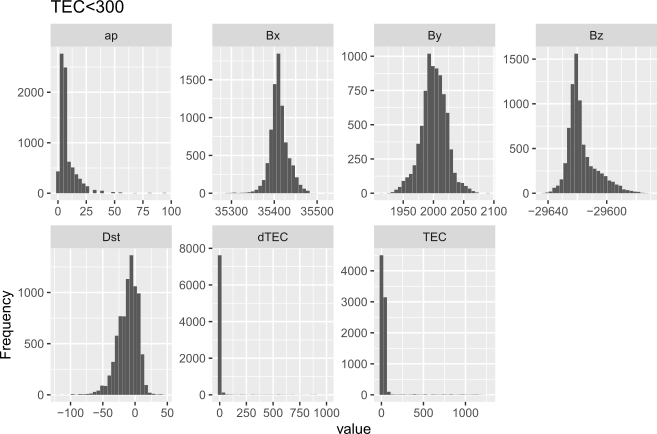
\includegraphics[width=0.9\linewidth]{300TEC_fix.png}
    \caption{Histograms of the relative frequency for all variables when the $TEC$ is less than $300$.}
    \label{fig:300TEC}
\end{figure}

\begin{table}[!ht]
    \centering
    \begin{tabular}{|c|c|c|c|c|c|}
        \hline
        & $TEC$ & $dTEC$ & $B_{x}$ & $B_{y}$ & $B_{z}$ \\ \hline
        Min. & $1.00$ & $0.01$ & $35268$ & $1900$ & $-29651$ \\ \hline
        $1^{st}$ Qu. & $7.26$ & $1.66$ & $35400$ & $1988$ & $-29623$ \\ \hline
        Median & $19.62$ & $3.13$ & $35410$ & $2001$ & $-29620$ \\ \hline
        Mean & $40.00$ & $15.88$ & $35412$ & $2001$ & $-29617$ \\ \hline
        $3^{rd}$ Qu. & $34.23$ & $6.49$ & $35423$ & $2015$ & $-29613$ \\ \hline
        Max. & $1288.00$ & $997.00$ & $35527$ & $2092$ & $-29570$ \\ \hline
    \end{tabular}
    \caption{The minimum, $1^{st}$ quartile, median, arithmetic mean, $3^{rd}$ quartile, and maximum values for all variables.}
    \label{tab:my_label}
\end{table}

\subsubsection{Data Pre-processing}
%\label{subsubsec:Pre-processing}

Data pre-processing is recommended to increase classification accuracy [30], so this step was also applied to the input data before training the models in this study. There are many ways to standardize data, such as minimum-maximum, normalization by decimal scaling, and Z-score [31]. Subtracting the mean and dividing by the variance for each feature are commonly used for Support Vector Machines (SVMs) [32] and other models tested in this study, so this approach was chosen. 

The values \textit{scale} and \textit{center} were used in the code for this study in the \textit{preProcess} parameter for the \textit{train} function from the \textit{caret} package developed for \textit{R}. The option \textit{center} subtracts the mean of each feature while \textit{center} divides by the standard deviation. 

\subsubsection{Training and Testing Dataset}
%\label{subsubsec:DataTrainTest}

The samples are divided into training and testing datasets as close as possible to a ratio of $80\%$ for training and $20\%$ for testing. During the division, the share of classes in the original data was taken into account, that is, the division was stratified by class so that an approximately equal ratio of classes was present in both the training data and the testing data, which is a feature of the \textit{createDataPartition} function from the \textit{caret} R library that was used [136, 137, 138].

\subsection{Performance Metrics}
%\label{subsec:Metrics}

\subsubsection{Confusion Matrix}
%\label{subsubsec:ConfusionMatrix}

The metrics and terminology used to evaluate the classifier performance were taken from the confusion matrix defined in the R function \textit{confusionMatrix} in the \textit{caret} library [139, 140, 141, 142, 143]. The confusion matrix is suitable for use in multiclass classification, which is the goal of this project. A confusion matrix is a table where the number of rows and columns corresponds to the number of classes. The cells report the number of samples in each class classified into any class. This enables a more detailed analysis than by observing the share of correct classifications, i.e. accuracy. Accuracy will give results that can lead us to a wrong conclusion if the data set is unbalanced, that is, if the numbers of observations in different classes vary significantly, which was the case in this paper, because out of a total of $1597$ samples, $1170$ of them belonged to the largest N class, and $3$ to the smallest E class.

If there are only two classes (Yes and No), the metrics are calculated using an example of a confusion matrix in Table~\ref{tab:cm}.

A true positive (TP) classification result correctly indicates that the sample belongs to the positive class.

A true negative (TN) classification result correctly indicates that the sample belongs to the negative class.
 
A false positive (FP) classification result or type I error, incorrectly indicates that the sample belongs to the positive class because it truly belongs to the negative class.

A false negative (FN) classification result or type II error, incorrectly indicates that the sample belongs to the negative class because it truly belongs to the positive class.

\begin{table}[!ht]
	\centering
	\begin{tabular}{|c|c|c|}
		\hline
		 & \multicolumn{2}{|c|}{Reference} \\ \hline
        Prediction & Yes & No \\ \hline
        Yes & TP & FP \\ \hline
        No & FN & TN \\ \hline
	\end{tabular}
	\caption{The confusion matrix for a two-class problem.}
	\label{tab:cm}
\end{table}

Sensitivity, recall, hit rate, or true positive rate (TPR), is calculated as $\mathrm{TP}/(\mathrm{TP}+\mathrm{FN})$, that is, the proportion of samples that are correctly classified as positive among all samples that truly belong to the positive class. Higher TPR values indicate better results for the positive class.

Specificity, selectivity, or true negative rate (TNR), is calculated using the expression $\mathrm{TN}/(\mathrm{TN}+\mathrm{FP})$, that is, the proportion of samples that are correctly classified as negative among all samples that truly belong to the negative class. Higher TNR values indicate better results for the negative class.

Prevalence is calculated as $(\mathrm{TP}+\mathrm{FN})/(\mathrm{TP}+\mathrm{FP}+\mathrm{FN}+\mathrm{TN})$ for the positive class, that is, the proportion of samples that truly belong to the positive class among all samples. Prevalence values other than an even split by the number of classes indicate a class imbalance.

Precision, or positive predictive value (PPV), is calculated as $\mathrm{TP}/(\mathrm{TP}+\mathrm{FP})$ for a two-class problem, i.e. the proportion of truly positive results among all samples classified as positive. 
Higher PPV values indicate better results for the positive class.

The negative predictive value (NPV) is calculated as $\mathrm{TN}/(\mathrm{TN}+\mathrm{FN})$ for a two-class problem, i.e. the share of truly negative results among all samples that are classified as negative. Higher NPV values indicate better results for the negative class.

The detection rate (DR) is calculated as $\mathrm{TP}/(\mathrm{TP}+\mathrm{FP}+\mathrm{FN}+\mathrm{TN})$ for the positive class, that is, that is, the proportion of samples that are correctly classified as positive among all samples.

The detection prevalence (DP) is calculated as $(\mathrm{TP}+\mathrm{FP})/(\mathrm{TP}+\mathrm{FP}+\mathrm{FN}+\mathrm{TN})$ for the positive class, that is, that is, the proportion of samples that are correctly or incorrectly classified as positive among all samples.

The accuracy (Acc) is calculated as $(\mathrm{TP} + \mathrm{TN}) / (\mathrm{TP} + \mathrm{TN} + \mathrm{FP} + \mathrm{FN})$, that is, the proportion of samples that are correctly classified among all samples.

Since accuracy is not usable in the case of unbalanced classes, balanced accuracy (BA) is introduced, which is calculated as $(\mathrm{TPR} + \mathrm{TNR}) / 2$ and is arithmetic mean TPR and TNR, which are respectively centered on the positive and on the negative class separately.

Another metric that can be used instead of accuracy to consider each class separately is the $F1$ score, i.e. the harmonic mean of PPV and TPR, equal to $2 \times (\mathrm{PPV} \times \mathrm{TPR}) / (\mathrm{PPV} + \mathrm{TPR}) = 2 \times \mathrm{TP} / (2 \times \mathrm{TP} + \mathrm{FP} + \mathrm{FN})$.

If there are more than two classes, results are calculated for each class separately by viewing that class as the positive class and samples of all other classes as negative, a "one versus all" approach.
The unweighted Kappa statistic and a \textit{p}-value from McNemar's test are also computed. McNemar's test produces NA values with sparse tables, such as the one in this experiment, so it was not included in the results.

A $95\%$ confidence interval for the accuracy rate is computed using \textit{binom.test} and a one-sided test [144, 145, 146, 147] to see if the accuracy is significantly larger than the "no information rate," which is the percentage of the largest class.

\subsubsection{The Binomial Test}
%\label{subsubsec:Binomial}

The binomial test [148, 149] for two classes is an exact test of the statistical significance of deviations from a theoretically expected distribution.

The binomial test is often utilized to validate a hypothesis about the probability ($\pi$) of success 
$H_{0}\colon \pi =\pi_{0}$, where users define $\pi_{0}$ between $0$ and $1$. The expected number of successes would be $n\pi_{0}$ if the null hypothesis $H_{0}$ were correct. If $k$ out of $n$ attempts are successful, the binomial distribution formula defines the probability in Equation~44.

\begin{equation}
	\Pr(X=k)={\binom{n}{k}}p^{k}(1-p)^{n-k}
	\quad\left(44\right)
\end{equation}

The probability of an outcome equally or more extreme than actual occurrences is used to calculate the $p$-value. This is a simple operation for a one-tailed test. 

Equation~45 contains the expression for the $p$-value when testing the hypothesis that $\pi <\pi_{0}$. We can use a range from $k$ to $n$ to test $\pi >\pi_{0}$.

\begin{equation}
	p=\sum_{i=0}^{k}\Pr(X=i)=\sum_{i=0}^{k}{\binom{n}{i}}\pi_{0}^{i}(1-\pi_{0})^{n-i}
	\quad\left(45\right)
\end{equation}

A binomial distribution isn't symmetric if $\pi_{0}\neq 0.5$, so calculating a $p$-value for a two-tailed test is not as simple. The $p$-value from the one-tailed test cannot be doubled to obtain the result since all events must be considered, including ones more extreme than previously seen. These extreme events are equally or less probable than $X=k$. Equation~46 denotes all such events. Equation~47 is used to compute the two-tailed $p$-value.

\begin{equation}
	{\mathcal{I}}=\{i\colon \Pr(X=i)\leq \Pr(X=k)\}
	\quad\left(46\right)
\end{equation}

\begin{equation}
	p=\sum_{i\in {\mathcal{I}}}\Pr(X=i)=\sum_{i\in {\mathcal{I}}}{\binom{n}{i}}\pi_{0}^{i}(1-\pi_{0})^{n-i}
	\quad\left(47\right)
\end{equation}

\subsubsection{Cohen's Kappa Coefficient}
%\label{subsubsec:kappa}

Cohen's kappa coefficient ($\kappa$, lowercase Greek kappa) indicates inter- and intra-rater reliability for classification [150]. As it accounts for random matches in ratings, it is a better metric than simply computing the percentage of agreement. Interpreting indices of agreement is not straightforward, and is still a point of contention among experts. Using disagreement instead of agreement in ratings might be simpler [151]. Galton was the first to use a statistic similar to Cohen's kappa in 1892 [152, 153]. Jacob Cohen formally described the kappa coefficient in 1960 in the journal "Educational and Psychological Measurement" [154].

Two raters group $N$ items into $C$ mutually exclusive classes, and Cohen's kappa measures their agreement. Equation~48 defines $\kappa$, where $p_{o}$ is the relative observed agreement among raters, and $p_{e}$ is the hypothetical probability of chance agreement. The observed data influences the computed probabilities of each observer randomly selecting each category.

\begin{equation}
	\kappa \equiv {\frac {p_{o}-p_{e}}{1-p_{e}}}=1-{\frac {1-p_{o}}{1-p_{e}}}
	\quad\left(48\right)
\end{equation}

If the raters completely align then $\kappa = 1$. When there is no agreement other than what would be expected by chance and is given by $p_{e}$, $\kappa = 0$. If $\kappa$ statistic is negative [155] there is no match between the raters, which can reflect a real tendency of the raters to give differing ratings.

Equation~49 is derived from the construction in Equation~50 and holds for $k$ categories with $N$ observations to categorize if $n_{k1}$ is the number of times rater $i$ predicted category $k$. In these equations, ${\widehat{p_{k12}}}$ is the estimated probability that both rater $1$ and rater $2$ will classify the same item as $k$, and ${\widehat {p_{k1}}}$ is the estimated probability that rater $1$ will classify an item as $k$. A similar claim can be made for rater $2$.

\begin{equation}
	p_{e}={\frac {1}{N^{2}}}\sum_{k}n_{k1}n_{k2}
	\quad\left(49\right)
\end{equation}

\begin{equation}
	p_{e}=\sum_{k}{\widehat {p_{k12}}}{\overset{\text{ind.}}{=}}\sum_{k}{\widehat {p_{k1}}}{\widehat {p_{k2}}}=\sum_{k}{\frac {n_{k1}}{N}}{\frac {n_{k2}}{N}}={\frac {1}{N^{2}}}\sum_{k}n_{k1}n_{k2}
	\quad\left(50\right)
\end{equation}

If ratings are independent Equation~51, can be used.

\begin{equation}
	\textstyle{\widehat{p_{k}}}=\sum_{k}{\widehat{p_{k1}}}{\widehat {p_{k2}}}
	\quad\left(51\right)
\end{equation}

Equation~52 is used to estimate the term $\widehat{p_{k1}}$ by using the number of items classified as $k$ by rater $1$ ($n_{k1}$) divided by the total items to classify ($N$).

\begin{equation}
	\widehat {p_{k1}}=\frac{n_{k1}}{N}
	\quad\left(52\right)
\end{equation}
 (and similarly for rater $2$).
 
Equation~53 contains the Cohen's Kappa formula [156] for the traditional confusion matrix for binary classifications in Table~\ref{tab:cm}.

\begin{equation}
	\kappa ={\frac{2\times (TP\times TN-FN\times FP)}{(TP+FP)\times (FP+TN)+(TP+FN)\times (FN+TN)}}
	\quad\left(53\right)
\end{equation}

In this scenario, Cohen's Kappa equals the Heidke skill score introduced by Myrick Haskell Doolittle in 1888 [157, 158].

\section{Research Results}
%\label{sec:Results}

The accuracy, CI, NIR, $p$-value, and Kappa statistic for each model when using all variables (all), all variables except $Dst$ (no $Dst$), all variables except $Dst$, $TEC$, and d$TEC$ (no $TEC$), only $B_{x}$, $B_{y}$, and $B_{z}$ (coord), only $B_{x}$, $B_{y}$, and $A_{p}$ ($x$ $y$ $A_{p}$), only $B_{x}$, $B_{z}$, and $A_{p}$ ($x$ $z$ $A_{p}$), or only $B_{y}$, $B_{z}$, and $A_{p}$ ($y$ $z$ $A_{p}$) is displayed in Table~\ref{tab:stats:reverse:all}, Table~\ref{tab:stats:reverse:no$Dst$}, Table~\ref{tab:stats:reverse:no$TEC$}, Table~\ref{tab:stats:reverse:coord}, Table~\ref{tab:stats:reverse:xyap}, Table~\ref{tab:stats:reverse:xzap}, and Table~\ref{tab:stats:reverse:yzap}.

\begin{table}[!ht]
	\centering
	\begin{tabular}{|c|c|c|c|c|c|}
		\hline
		Model & Acc & $95\%$ CI & NIR & $p$-value & Kappa \\ \hline
		svmPoly & $0.7672$ & $(0.7457, 0.7877)$ & $0.7322$ & $0.0007444$ & $0.3607$ \\ \hline
		C5.0 & $1$ & $(0.9977, 1)$ & $0.7322$ & $< 2.2 \times {10}^{-16}$ & $1$ \\ \hline
		nb & $0.9912$ & $(0.9853, 0.9952)$ & $0.7322$ & $< 2.2 \times {10}^{-16}$ & $0.9787$ \\ \hline
		nnet & $1$ & $(0.9977, 1)$ & $0.7322$ & $< 2.2 \times {10}^{-16}$ & $1$ \\ \hline
		pls & $0.9086$ & $(0.8934, 0.9223)$ & $0.7322$ & $< 2.2 \times {10}^{-16}$ & $0.7489$ \\ \hline
		fda & $0.9199$ & $(0.9055, 0.9327)$ & $0.7322$ & $< 2.2 \times {10}^{-16}$ & $0.8017$ \\ \hline
		pcaNNet & $0.9975$ & $(0.9936, 0.9993)$ & $0.7322$ & $< 2.2 \times {10}^{-16}$ & $0.9939$ \\ \hline
	\end{tabular}
	\caption{The accuracy, CI, NIR, $p$-value, and Kappa statistic for each model when using all variables as input.}
	\label{tab:stats:reverse:all}
\end{table}

\begin{table}[!ht]
	\centering
	\begin{tabular}{|c|c|c|c|c|c|}
		\hline
		Model & Acc & $95\%$ CI & NIR & $p$-value & Kappa \\ \hline
		svmPoly & $0.7284$ & $(0.7059, 0.7501)$ & $0.7322$ & $0.6447$ & $0.1137$ \\ \hline
		C5.0 & $0.8492$ & $(0.8307, 0.8664)$ & $0.7322$ & $< 2.2 \times {10}^{-16}$ & $0.6165$ \\ \hline
		nb & $0.9906$ & $(0.9846, 0.9947)$ & $0.7322$ & $< 2.2 \times {10}^{-16}$ & $0.9771$ \\ \hline
		nnet & $1$ & $(0.9977, 1)$ & $0.7322$ & $< 2.2 \times {10}^{-16}$ & $1$ \\ \hline
		pls & $0.7929$ & $(0.7722, 0.8125)$ & $0.7322$ & $1.104e-08$ & $0.3635$ \\ \hline
		fda & $0.8141$ & $(0.7942, 0.8329)$ & $0.7322$ & $9.859e-15$ & $0.5064$ \\ \hline
		pcaNNet & $0.8436$ & $(0.8248, 0.861)$ & $0.7322$ & $< 2.2 \times {10}^{-16}$ & $0.5868$ \\ \hline
	\end{tabular}
	\caption{The accuracy, CI, NIR, $p$-value, and Kappa statistic for each model when using all variables except $Dst$ as input.}
	\label{tab:stats:reverse:no$Dst$}
\end{table}

\begin{table}[!ht]
	\centering
	\begin{tabular}{|c|c|c|c|c|c|}
		\hline
		Model & Acc & $95\%$ CI & NIR & $p$-value & Kappa \\ \hline
		svmPoly & $0.7378$ & $(0.7155, 0.7592)$ & $0.7322$ & $0.3168$ & $0.1066$ \\ \hline
		C5.0 & $0.8448$ & $(0.8261, 0.8622)$ & $0.7322$ & $< 2.2 \times {10}^{-16}$ & $0.5882$ \\ \hline
		nb & $1$ & $(0.9977, 1)$ & $0.7322$ & $< 2.2 \times {10}^{-16}$ & $1$ \\ \hline
		nnet & $1$ & $(0.9977, 1)$ & $0.7322$ & $< 2.2 \times {10}^{-16}$ & $1$ \\ \hline
		pls & $0.7922$ & $(0.7715, 0.8119)$ & $0.7322$ & $1.556e-08$ & $0.3634$ \\ \hline
		fda & $0.8166$ & $(0.7968, 0.8353)$ & $0.7322$ & $1.416e-15$ & $0.5092$ \\ \hline
		pcaNNet & $0.8379$ & $(0.8189, 0.8557)$ & $0.7322$ & $< 2.2 \times {10}^{-16}$ & $0.5647$ \\ \hline
	\end{tabular}
	\caption{The accuracy, CI, NIR, $p$-value, and Kappa statistic for each model when using all variables except $Dst$, $TEC$, and d$TEC$ as input.}
	\label{tab:stats:reverse:no$TEC$}
\end{table}

\begin{table}[!ht]
	\centering
	\begin{tabular}{|c|c|c|c|c|c|}
		\hline
		Model & Acc & $95\%$ CI & NIR & $p$-value & Kappa \\ \hline
		svmPoly & $0.7409$ & $(0.7187, 0.7623)$ & $0.7322$ & $0.2234$ & $0.0887$ \\ \hline
		C5.0 & $0.826$ & $(0.8065, 0.8443)$ & $0.7322$ & $< 2.2 \times {10}^{-16}$ & $0.5208$ \\ \hline
		nb & $1$ & $(0.9977, 1)$ & $0.7322$ & $< 2.2 \times {10}^{-16}$ & $1$ \\ \hline
		nnet & $1$ & $(0.9977, 1)$ & $0.7322$ & $< 2.2 \times {10}^{-16}$ & $1$ \\ \hline
		pls & $0.7835$ & $(0.7625, 0.8035)$ & $0.7322$ & $1.284e-06$ & $0.298$ \\ \hline
		fda & $0.7979$ & $(0.7773, 0.8173)$ & $0.7322$ & $6.224e-10$ & $0.4541$ \\ \hline
		pcaNNet & $0.8254$ & $(0.8059, 0.8437)$ & $0.7322$ & $< 2.2 \times {10}^{-16}$ & $0.5242$ \\ \hline
	\end{tabular}
	\caption{The accuracy, CI, NIR, $p$-value, and Kappa statistic for each model when using only $B_{x}$, $B_{y}$, and $B_{z}$ as input.}
	\label{tab:stats:reverse:coord}
\end{table}

\begin{table}[!ht]
	\centering
	\begin{tabular}{|c|c|c|c|c|c|}
		\hline
		Model & Acc & $95\%$ CI & NIR & $p$-value & Kappa \\ \hline
		svmPoly & $0.7416$ & $(0.7193, 0.7629)$ & $0.7322$ & $0.2068$ & $0.103$ \\ \hline
		C5.0 & $0.8292$ & $(0.8098, 0.8473)$ & $0.7322$ & $< 2.2 \times {10}^{-16}$ & $0.5386$ \\ \hline
		nb & $1$ & $(0.9977, 1)$ & $0.7322$ & $< 2.2 \times {10}^{-16}$ & $1$ \\ \hline
		nnet & $1$ & $(0.9977, 1)$ & $0.7322$ & $< 2.2 \times {10}^{-16}$ & $1$ \\ \hline
		pls & $0.781$ & $(0.7599, 0.801)$ & $0.7322$ & $3.978e-06$ & $0.3153$ \\ \hline
		fda & $0.8204$ & $(0.8007, 0.8389)$ & $0.7322$ & $< 2.2 \times {10}^{-16}$ & $0.5099$ \\ \hline
		pcaNNet & $0.8367$ & $(0.8176, 0.8545)$ & $0.7322$ & $< 2.2 \times {10}^{-16}$ & $0.5579$ \\ \hline
	\end{tabular}
	\caption{The accuracy, CI, NIR, $p$-value, and Kappa statistic for each model when using only $B_{x}$, $B_{y}$, and $A_{p}$ as input.}
	\label{tab:stats:reverse:xyap}
\end{table}

\begin{table}[!ht]
	\centering
	\begin{tabular}{|c|c|c|c|c|c|}
		\hline
		Model & Acc & $95\%$ CI & NIR & $p$-value & Kappa \\ \hline
		svmPoly & $0.739$ & $(0.7168, 0.7604)$ & $0.7322$ & $0.2775$ & $0.1013$ \\ \hline
		C5.0 & $0.8104$ & $(0.7903, 0.8293)$ & $0.7322$ & $1.602e-13$ & $0.4714$ \\ \hline
		nb & $1$ & $(0.9977, 1)$ & $0.7322$ & $< 2.2 \times {10}^{-16}$ & $1$ \\ \hline
		nnet & $1$ & $(0.9977, 1)$ & $0.7322$ & $< 2.2 \times {10}^{-16}$ & $1$ \\ \hline
		pls & $0.7735$ & $(0.7521, 0.7938)$ & $0.7322$ & $8.468e-05$ & $0.2742$ \\ \hline
		fda & $0.7979$ & $(0.7773, 0.8173)$ & $0.7322$ & $6.224e-10$ & $0.4343$ \\ \hline
		pcaNNet & $0.8148$ & $(0.7948, 0.8335)$ & $0.7322$ & $6.107e-15$ & $0.4948$ \\ \hline
	\end{tabular}
	\caption{The accuracy, CI, NIR, $p$-value, and Kappa statistic for each model when using only $B_{x}$, $B_{z}$, and $A_{p}$ as input.}
	\label{tab:stats:reverse:xzap}
\end{table}

\begin{table}[!ht]
	\centering
	\begin{tabular}{|c|c|c|c|c|c|}
		\hline
		Model & Acc & $95\%$ CI & NIR & $p$-value & Kappa \\ \hline
		svmPoly & $0.7347$ & $(0.7123, 0.7562)$ & $0.7322$ & $0.4233$ & $0.0251$ \\ \hline
		C5.0 & $0.7866$ & $(0.7657, 0.8065)$ & $0.7322$ & $2.88e-07$ & $0.3926$ \\ \hline
		nb & $0.9987$ & $(0.9955, 0.9998)$ & $0.7322$ & $< 2.2 \times {10}^{-16}$ & $0.9969$ \\ \hline
		nnet & $1$ & $(0.9977, 1)$ & $0.7322$ & $< 2.2 \times {10}^{-16}$ & $1$ \\ \hline
		pls & $0.7566$ & $(0.7348, 0.7774)$ & $0.7322$ & $0.01419$ & $0.2075$ \\ \hline
		fda & $0.7672$ & $(0.7457, 0.7877)$ & $0.7322$ & $0.0007444$ & $0.3367$ \\ \hline
		pcaNNet & $0.7797$ & $(0.7586, 0.7998)$ & $0.7322$ & $6.857e-06$ & $0.3878$ \\ \hline
	\end{tabular}
	\caption{The accuracy, CI, NIR, $p$-value, and Kappa statistic for each model when using only $B_{y}$, $B_{z}$, and $A_{p}$ as input.}
	\label{tab:stats:reverse:yzap}
\end{table}

The execution time in seconds calculated using the R \textit{system.time} function [159] for each model when using different combinations of variables as input is displayed in Table~\ref{tab:time:total}. The experiment was run on Windows 11 using R Studio version 2024.04.2+764 and R version 4.4.1, the AMD Radeon RX 6600 GPU, 16GB of RAM, and the AMD Ryzen 5 PRO 4650G CPU with 6 cores.

\begin{table}[!ht]
	\centering
	\begin{tabular}{|c|c|c|c|c|c|c|c|}
		\hline
		Model & svmPoly & C5.0 & nb & nnet & pls & fda & pcaNNet \\ \hline
		all & $103.52$ & $169.28$ & $192.05$ & $494.53$ & $49.99$ & $51.57$ & $291.98$ \\ \hline
		no $Dst$ & $276.24$ & $592.32$ & $175.38$ & $479.67$ & $42.89$ & $49.34$ & $305.16$ \\ \hline
		no $TEC$ & $285.58$ & $393.72$ & $137.99$ & $453.82$ & $33.11$ & $60.53$ & $294.58$ \\ \hline
		coord & $331.13$ & $277.63$ & $118.86$ & $441.37$ & $22.28$ & $67.94$ & $294.97$ \\ \hline
		$x$ $y$ $A_{p}$ & $319.97$ & $295.20$ & $121.73$ & $465.61$ & $26.72$ & $70.97$ & $302.48$ \\ \hline
		$x$ $z$ $A_{p}$ & $348.47$ & $259.81$ & $121.05$ & $475.05$ & $25.56$ & $76.04$ & $321.05$ \\ \hline
		$y$ $z$ $A_{p}$ & $416.75$ & $277.62$ & $124.02$ & $489.08$ & $29.89$ & $95.64$ & $345.05$ \\ \hline
	\end{tabular}
	\caption{The execution time in seconds for each model when using different combinations of variables as input.}
	\label{tab:time:total}
\end{table}

\subsection{A Comprehensive Analysis of the Naive Bayes Model}
%\label{subsec:AnalysisNB}

The confusion matrix and the performance indicators derived from it when using the Naive Bayes model and all input variables are depicted in Table~\ref{tab:cm:all:nb} and Table~\ref{tab:cs:reverse:all:nb}. The same values when using all input variables except $Dst$ are marked in Table~\ref{tab:cm:no$Dst$:nb} and Table~\ref{tab:cs:reverse:no$Dst$:nb}, and Table~\ref{tab:cm:yzap:nb} and Table~\ref{tab:cs:reverse:yzap:nb} when using only $B_{y}$, $B_{z}$, and $A_{p}$ variables as input. These results are displayed since the Naive Bayes model has low computational load and high accuracy. The combinations of input variables that produced a $100\%$ accuracy when used for the Naive Bayes model were not included since there are no errors in classification.

\begin{table}[!ht]
	\centering
	\begin{tabular}{|c|c|c|c|c|c|}
		\hline
		 & \multicolumn{5}{|c|}{Reference} \\ \hline
		 Prediction & E & N & P & R & T \\ \hline
		 E & $3$ & $1$ & $0$ & $0$ & $0$ \\ \hline
		 N & $0$ & $1161$ & $1$ & $1$ & $0$ \\ \hline
		 P & $0$ & $5$ & $26$ & $2$ & $0$ \\ \hline
		 R & $0$ & $3$ & $0$ & $375$ & $0$ \\ \hline
		 T & $0$ & $0$ & $0$ & $1$ & $19$ \\ \hline
	\end{tabular}
	\caption{The confusion matrix for the Naive Bayes model when using all variables as input.}
	\label{tab:cm:all:nb}
\end{table}

\begin{table}[!ht]
	\centering
	\begin{tabular}{|c|c|c|c|c|c|}
		\hline
		 & \multicolumn{5}{c|}{Class} \\ \hline
		Statistics & E & N & P & R & T \\ \hline
		Sensitivity & $100\%$ & $99.23\%$ & $96.296\%$ & $98.94\%$ & $100\%$ \\ \hline
		Specificity & $99.9373\%$ & $99.53\%$ & $99.554\%$ & $99.75\%$ & $99.937\%$ \\ \hline
		PPV & $75\%$ & $99.83\%$ & $78.788\%$ & $99.21\%$ & $95\%$ \\ \hline
		NPV & $100\%$ & $97.93\%$ & $99.936\%$ & $99.67\%$ & $100\%$ \\ \hline
		DR & $0.1877\%$ & $72.65\%$ & $1.627\%$ & $23.47\%$ & $1.189\%$ \\ \hline
		DP & $0.2503\%$ & $72.78\%$ & $2.065\%$ & $23.65\%$ & $1.252\%$ \\ \hline
		BA & $99.9687\%$ & $99.38\%$ & $97.925\%$ & $99.35\%$ & $99.968\%$ \\ \hline
	\end{tabular}
	\caption{The performance indicators derived from the confusion matrix for the Naive Bayes model when using all variables as input.}
	\label{tab:cs:reverse:all:nb}
\end{table}

\begin{table}[!ht]
	\centering
	\begin{tabular}{|c|c|c|c|c|c|}
		\hline
		 & \multicolumn{5}{|c|}{Reference} \\ \hline
		 Prediction & E & N & P & R & T \\ \hline
		 E & $3$ & $1$ & $0$ & $0$ & $0$ \\ \hline
		 N & $0$ & $1161$ & $2$ & $2$ & $0$ \\ \hline
		 P & $0$ & $5$ & $25$ & $1$ & $0$ \\ \hline
		 R & $0$ & $3$ & $0$ & $375$ & $0$ \\ \hline
		 T & $0$ & $0$ & $0$ & $1$ & $19$ \\ \hline
	\end{tabular}
	\caption{The confusion matrix for the Naive Bayes model when using all variables except $Dst$ as input.}
	\label{tab:cm:no$Dst$:nb}
\end{table}

\begin{table}[!ht]
	\centering
	\begin{tabular}{|c|c|c|c|c|c|}
		\hline
		 & \multicolumn{5}{c|}{Class} \\ \hline
		Statistics & E & N & P & R & T \\ \hline
		Sensitivity & $100\%$ & $99.23\%$ & $92.593\%$ & $98.94\%$ & $100\%$ \\ \hline
		Specificity & $99.9373\%$ & $99.07\%$ & $99.618\%$ & $99.75\%$ & $99.937\%$ \\ \hline
		PPV & $75\%$ & $99.66\%$ & $80.645\%$ & $99.21\%$ & $95\%$ \\ \hline
		NPV & $100\%$ & $97.92\%$ & $99.872\%$ & $99.67\%$ & $100\%$ \\ \hline
		DR & $0.1877\%$ & $72.65\%$ & $1.564\%$ & $23.47\%$ & $1.189\%$ \\ \hline
		DP & $0.2503\%$ & $72.9\%$ & $1.94\%$ & $23.65\%$ & $1.252\%$ \\ \hline
		BA & $99.9687\%$ & $99.15\%$ & $96.105\%$ & $99.35\%$ & $99.968\%$ \\ \hline
	\end{tabular}
	\caption{The performance indicators derived from the confusion matrix for the Naive Bayes model when using all variables except $Dst$ as input.}
	\label{tab:cs:reverse:no$Dst$:nb}
\end{table}

\begin{table}[!ht]
	\centering
	\begin{tabular}{|c|c|c|c|c|c|}
		\hline
		 & \multicolumn{5}{|c|}{Reference} \\ \hline
		 Prediction & E & N & P & R & T \\ \hline
		 E & $2$ & $0$ & $0$ & $0$ & $0$ \\ \hline
		 N & $1$ & $1170$ & $1$ & $0$ & $0$ \\ \hline
		 P & $0$ & $0$ & $26$ & $0$ & $0$ \\ \hline
		 R & $0$ & $0$ & $0$ & $379$ & $0$ \\ \hline
		 T & $0$ & $0$ & $0$ & $0$ & $19$ \\ \hline
	\end{tabular}
	\caption{The confusion matrix for the Naive Bayes model when using only $B_{y}$, $B_{z}$, and $A_{p}$ as input.}
	\label{tab:cm:yzap:nb}
\end{table}

\begin{table}[!ht]
	\centering
	\begin{tabular}{|c|c|c|c|c|c|}
		\hline
		 & \multicolumn{5}{c|}{Class} \\ \hline
		Statistics & E & N & P & R & T \\ \hline
		Sensitivity & $66.6667\%$ & $100\%$ & $96.296\%$ & $100\%$ & $100\%$ \\ \hline
		Specificity & $100\%$ & $99.53\%$ & $100\%$ & $100\%$ & $100\%$ \\ \hline
		PPV & $100\%$ & $99.83\%$ & $100\%$ & $100\%$ & $100\%$ \\ \hline
		NPV & $99.9373\%$ & $100\%$ & $99.936\%$ & $100\%$ & $100\%$ \\ \hline
		DR & $0.1252\%$ & $73.22\%$ & $1.627\%$ & $23.72\%$ & $1.189\%$ \\ \hline
		DP & $0.1252\%$ & $73.34\%$ & $1.627\%$ & $23.72\%$ & $1.189\%$ \\ \hline
		BA & $83.3333\%$ & $99.77\%$ & $98.148\%$ & $100\%$ & $100\%$ \\ \hline
	\end{tabular}
	\caption{The performance indicators derived from the confusion matrix for the Naive Bayes model when using only $B_{y}$, $B_{z}$, and $A_{p}$ as input.}
	\label{tab:cs:reverse:yzap:nb}
\end{table}

\section{Discussion}
%\label{sec:Discussion}

The Neural Network model has the highest execution time for any subset of the input variables due to its complexity and extensive training, evident from the data in Table~\ref{tab:time:total}. However, in each case, it achieved a $100\%$ accuracy, which is shown in Table~\ref{tab:stats:reverse:all}, Table~\ref{tab:stats:reverse:no$Dst$}, Table~\ref{tab:stats:reverse:no$TEC$}, Table~\ref{tab:stats:reverse:coord}, Table~\ref{tab:stats:reverse:xyap}, Table~\ref{tab:stats:reverse:xzap}, and Table~\ref{tab:stats:reverse:yzap}. The Naive Bayes model has the second highest accuracy, over $99\%$. The Naive Bayes model achieved a $100\%$ accuracy, except when using all input variables, all input variables except $Dst$, or only $B_{y}$, $B_{z}$, and $A_{p}$. The difference in accuracy between the Neural Network and the Naive Bayes model is negligible, and the training time for the Neural Network model is more than twice as long. Despite their simple design and seemingly oversimplified assumptions, Naive Bayes classifiers have performed quite well in many complex real-world situations. In 2004., an analysis of the Bayesian classification problem showed that there are reasonable theoretical reasons for the seemingly incredible performance of Naive Bayesian classifiers [58].

All other models fail to achieve an accuracy over $90\%$, except when using all input variables, including $Dst$. The $Dst$ class was derived by thresholding the continuous $Dst$ value and discretizing it by converting it to a single character. This labeling method explains the increase in accuracy when adding the $Dst$ input variable in all except the two best-performing models. For example, the C5.0 model using Decision Trees did not consider any variable except $Dst$ when included in the input, indicated by a $100\%$ variable importance. The svmPoly model is consistently the worst-performing for any subset of input variables, never achieving an accuracy over $80\%$. None of the models achieved an accuracy under $70\%$, so they were all moderately successful.

When studying the performance of the Naive Bayes model by individual class in Table~\ref{tab:cm:all:nb}, Table~\ref{tab:cs:reverse:all:nb}, Table~\ref{tab:cm:no$Dst$:nb}, Table~\ref{tab:cs:reverse:no$Dst$:nb}, Table~\ref{tab:cm:yzap:nb} and Table~\ref{tab:cs:reverse:yzap:nb}, samples of the T class are all correctly classified, but the testing is less extensive since it is the second smallest class. Samples of the R class are sometimes erroneously assigned to the N, P, or less commonly the T class. Samples of the P class are rarely mistaken for the N class. Two of the most common misclassifications were assigning samples of the N class to the P or R classes. This is due to the largest number of samples in the N class between the P and R classes with the narrowest $Dst$ range. Samples of the N class are least often included in the E class, whose range is the furthest apart from the N class. A sample of the E class was attributed to the N class only once. The E class is the smallest with only three samples, which must be accounted for when interpreting these results.

\section{Conclusion}
%\label{sec:Conclusion}

The results indicate that even a limited subset of variables, including coordinates ad $A_{p}$, available on simple devices such as smartphones, without measuring $TEC$ and calculating $Dst$, can be successfully utilized to construct a simple and efficient model using a Naive Bayes classifier to determine $Dst$ classes. The Neural Network model was marginally more accurate. However, the training time and model size were inappropriate for developing a new model with additional data or utilizing the model in practice.

% conflicts of interest

\section*{Declaration of competing interest}

The authors declare no conflict of interest.

\section*{CRediT authorship contribution statement}

\textbf{Lucija \v{Z}u\v{z}i\'{c}:} Conceptualization, Methodology, Software, Validation, Investigation, Data Curation, Writing -- Original Draft, Visualization. 

\textbf{Deni Klen:} Conceptualization, Methodology, Software, Validation, Investigation, Data Curation, Writing -- Original Draft, Visualization. 

\textbf{Teodor B. Iliev:} Conceptualization,  Validation, Formal analysis, Investigation, Resources, Writing -- Original Draft, Writing -- Review \& Editing, Supervision. 

\textbf{Renato Filjar:} Conceptualization, Methodology, Validation, Formal analysis, Investigation, Resources, Writing -- Original Draft, Writing -- Review \& Editing, Supervision, Project administration, Funding acquisition.

% acknowledgment

\section*{Funding}

This work was fully supported by

% Adding a bibliography if citations are used in the report
\section{Bibliography}
%\label{sec:Bibliography}
[1] R. Filjar, “An application-centred resilient GNSS position estimation algorithm based on positioning environment conditions awareness,” in Proceedings of the 2022 International Technical Meeting of The Institute of Navigation, 2022, pp. 1123–1136.
[2] R. Filjar, I. Hedji, J. Prpić-Oršić, and T. Iliev, “An Ambient Adaptive Global Navigation Satellite System Total Electron Content Predictive Model for Short-Term Rapid Geomagnetic Storm Events,” Remote Sensing, vol. 16, no. 16, p. 3051, 2024.
[3] K. Davies, Ionospheric Radio. Institution of Engineering & Technology, 1990. [Online] . Available: https://books.google.hr/books?id=qdWUKSj5PCcC
[4] M. Filić and R. Filjar, “modelling the relation between GNSS positioning performance degradation, and space weather and ionospheric conditions using RReliefF features selection,” in ION GNSS+ 2018 Meeting, 2018, pp. 1999–2006.
[5] J. J. Spilker Jr, P. Axelrad, B. W. Parkinson, and P. Enge, Global positioning system: theory and applications, volume I. American Institute of Aeronautics, 1996.
[6] A. Oxley, Uncertainties in GPS Positioning: A mathematical discourse. Academic Press, 2017.
[7] N. Sikirica, F. Dimc, O. Jukic, T. B. Iliev, D. Spoljar, and R. Filjar, “A Risk Assessment of Geomagnetic Conditions Impact on GPS Positioning Accuracy Degradation in Tropical Regions Using Dst Index,” in Proceedings of the 2021 International Technical Meeting of The Institute of Navigation, 2021, pp. 606–615.
[8] R. Natras, B. Soja, and M. Schmidt, “Ensemble machine learning of random forest, AdaBoost and XGBoost for vertical total electron content forecasting,” Remote Sensing, vol. 14, no. 15, p. 3547, 2022.
[9] R. Natras et al., “Regional ionosphere delay models based on CORS data and machine learning,” NAVIGATION: Journal of the Institute of Navigation, vol. 70, no. 3, 2023.
[10] R. Filjar, I. Sklebar, and M. Horvat, “A COMPARISON OF MACHINE LEARNING-BASED INDIVIDUAL MOBILITY CLASSIFICATION MODELS DEVELOPED ON SENSOR READINGS FROM LOOSELY ATTACHED SMARTPHONES.,” Komunikácie, vol. 22, no. 4, 2020.
[11] R.-E. Fan, K.-W. Chang, C.-J. Hsieh, X.-R. Wang, and C.-J. Lin, “LIBLINEAR: a library for large linear classification,” Journal of Machine Learning Research, vol. 9, pp. 1871–1874, Aug. 2008, doi: 10.1145/1390681.1442794.
[12] I. B. Mohamad and D. Usman, “Standardization and its effects on K-means clustering algorithm,” Research Journal of Applied Sciences, Engineering and Technology, vol. 6, no. 17, pp. 3299–3303, Sep. 2013.
[13] P. G. Fennell, Z. Zuo, and K. Lerman, “Predicting and explaining behavioral data with structured feature space decomposition,” EPJ Data Sci., vol. 8, no. 1, Dec. 2019.
[14] M. Kuhn, Applied predictive modeling. Springer, 2013.
[15] M. Kuhn, The caret Package — topepo.github.io. https://topepo.github.io/caret/, 2024. [Online] . Available: https://topepo.github.io/caret/
[16] RCoreTeam, R: The R Project for Statistical Computing — r-project.org. https://www.r-project.org/, 2024. [Online] . Available: https://www.r-project.org/
[17] MIT, Explained: Neural networks — news.mit.edu. https://news.mit.edu/2017/explained-neural-networks-deep-learning-0414, 2017. [Online] . Available: https://news.mit.edu/2017/explained-neural-networks-deep-learning-0414
[18] A. Brahme, Comprehensive biomedical physics. Newnes, 2014.
[19] J. D. Olden and D. A. Jackson, “Illuminating the ‘black box’: a randomization approach for understanding variable contributions in artificial neural networks,” Ecological modelling, vol. 154, no. 1–2, pp. 135–150, 2002.
[20] S. L. Özesmi and U. Özesmi, “An artificial neural network approach to spatial habitat modelling with interspecific interaction,” Ecological modelling, vol. 116, no. 1, pp. 15–31, 1999.
[21] C. Bishop, Pattern Recognition and Machine Learning. Springer, 2006.
[22] V. Vapnik, The nature of statistical learning theory. Springer science & business media, 2013.
[23] I. Goodfellow, Deep learning. MIT press, 2016.
[24] P. Probst, A.-L. Boulesteix, and B. Bischl, “Tunability: Importance of hyperparameters of machine learning algorithms,” Journal of Machine Learning Research, vol. 20, no. 53, pp. 1–32, 2019.
[25] B. Zoph, “Neural architecture search with reinforcement learning,” arXiv preprint arXiv:1611.01578, 2016.
[26] H. Jin, Q. Song, and X. Hu, “Auto-keras: An efficient neural architecture search system,” in Proceedings of the 25th ACM SIGKDD international conference on knowledge discovery & data mining, 2019, pp. 1946–1956.
[27] M. Claesen and B. De Moor, “Hyperparameter search in machine learning,” arXiv preprint arXiv:1502.02127, 2015.
[28] Y. H. Liu, Python Machine Learning by Example: Build Intelligent Systems Using Python, TensorFlow 2, PyTorch, and Scikit-Learn. Packt Publishing Ltd, 2020.
[29] B. E. Boser, I. M. Guyon, and V. N. Vapnik, “A training algorithm for optimal margin classifiers,” Jul. 1992.
[30] C. Cortes and V. Vapnik, “Support-vector networks,” Mach. Learn., vol. 20, no. 3, pp. 273–297, Sep. 1995.
[31] A. Ben-Hur, D. Horn, H. Siegelmann, and V. Vapnik, “Support Vector Clustering,” Journal of Machine Learning Research, vol. 2, pp. 125–137, Nov. 2001, doi: 10.1162/15324430260185565.
[32] D. Meyer, F. Leisch, and K. Hornik, “The support vector machine under test,” Neurocomputing, vol. 55, no. 1–2, pp. 169–186, Sep. 2003.
[33] scikit-learn developers, 1.4. Support Vector Machines — scikit-learn.org. http://scikit-learn.org/stable/modules/svm.html, 2023. [Online] . Available: http://scikit-learn.org/stable/modules/svm.html
[34] T. Hastie, S. Rosset, J. Zhu, and H. Zou, “Multi-class AdaBoost,” Stat. Interface, vol. 2, no. 3, pp. 349–360, 2009.
[35] W. H. Press, S. A. Teukolsky, W. T. Vetterling, and B. P. Flannery, Numerical recipes 3rd edition, Third. Cambridge, England: Cambridge University Press, 2007.
[36] T. Joachims, “Text categorization with Support Vector Machines: Learning with many relevant features,” in Machine Learning: ECML-98, Berlin, Heidelberg: Springer Berlin Heidelberg, 1998, pp. 137–142.
[37] S. S. Pradhan, W. H. Ward, K. Hacioglu, J. H. Martin, and D. Jurafsky, “Shallow Semantic Parsing using Support Vector Machines,” in Proceedings of the Human Language Technology Conference of the North American Chapter of the Association for Computational Linguistics: HLT-NAACL 2004, 2004, pp. 233–240. [Online] . Available: https://aclanthology.org/N04-1030
[38] A. Laurent, O. Strauss, B. Bouchon-Meunier, and R. R. Yager, Information Processing and Management of Uncertainty in Knowledge-Based Systems. Springer, 2014, p. 442.
[39] L. Barghout, “Spatial-taxon information granules as used in iterative fuzzy-decision-making for image segmentation,” in Studies in Big Data, Cham: Springer International Publishing, 2015, pp. 285–318.
[40] A. Maity, “Supervised classification of RADARSAT-2 polarimetric data for different land features,” arXiv preprint arXiv:1608.00501, Aug. 2016.
[41] D. Decoste and B. Schölkopf, “Training Invariant Support Vector Machines,” Mach. Learn., vol. 46, no. 1/3, pp. 161–190, 2002.
[42] D. S. Maitra, U. Bhattacharya, and S. K. Parui, “CNN based common approach to handwritten character recognition of multiple scripts,” Aug. 2015.
[43] B. Gaonkar and C. Davatzikos, “Analytic estimation of statistical significance maps for support vector machine based multi-variate image analysis and classification,” Neuroimage, vol. 78, pp. 270–283, Sep. 2013.
[44] R. Cuingnet et al., “Spatial regularization of SVM for the detection of diffusion alterations associated with stroke outcome,” Med. Image Anal., vol. 15, no. 5, pp. 729–737, Oct. 2011.
[45] A. Statnikov, D. Hardin, and C. Aliferis, “Using SVM Weight-Based Methods to Identify Causally Relevant and Non-Causally Relevant Variables,” Sign, vol. 1, Jan. 2006.
[46] M. A. Aizerman, E. A. Braverman, and L. Rozonoer, “Theoretical foundations of the potential function method in pattern recognition learning,” in Automation and Remote Control, 1964, no. 25, pp. 821–837.
[47] C. Jin and L. Wang, “Dimensionality dependent PAC-Bayes margin bound,” Advances in Neural Information Processing Systems, vol. 2, pp. 1034–1042, Jan. 2012.
[48] C.-W. Hsu, C.-C. Chang, and C.-J. Lin, “A Practical Guide to Support Vector Classification,” Department of Computer Science, National Taiwan University, techreport, 2003. [Online] . Available: http://www.csie.ntu.edu.tw/~cjlin/papers.html
[49] M. Studer, G. Ritschard, A. Gabadinho, and N. S. Müller, “Discrepancy analysis of state sequences,” Sociol. Methods Res., vol. 40, no. 3, pp. 471–510, Aug. 2011.
[50] X. Wu et al., “Top 10 algorithms in data mining,” Knowl. Inf. Syst., vol. 14, no. 1, pp. 1–37, Jan. 2008.
[51] L. Rokach and O. Maimon, Data mining with decision trees. World Scientific Publishing Company, 2014.
[52] S. Shalev-Shwartz and S. Ben-David, “Decision Trees,” in Understanding Machine Learning: From Theory to Algorithms, Cambridge University Press, 2014, pp. 212–218. doi: 10.1017/CBO9781107298019.019.
[53] J. R. Quinlan, “Induction of decision trees,” Mach. Learn., vol. 1, no. 1, pp. 81–106, Mar. 1986.
[54] L. Rokach and O. Maimon, “Top-down induction of decision trees classifiers—A survey,” IEEE Trans. Syst. Man Cybern. C Appl. Rev., vol. 35, no. 4, pp. 476–487, Nov. 2005.
[55] A. McCallum, Graphical Models Lecture 2: Bayesian Network Representation. https://people.cs.umass.edu/ mccallum/courses/gm2011/02-bn-rep.pdf, 2011. [Online] . Available: https://people.cs.umass.edu/ mccallum/courses/gm2011/02-bn-rep.pdf
[56] S. Russell and P. Norvig, Artificial intelligence, Second. Upper Saddle River, NJ: Pearson, 1999.
[57] D. J. Hand and K. Yu, “Idiot’s Bayes: Not So Stupid after All?,” Int. Stat. Rev., vol. 69, no. 3, p. 385, Dec. 2001.
[58] H. Zhang, “The Optimality of Naive Bayes,” in Proceedings of the Seventeenth International Florida Artificial Intelligence Research Society Conference, FLAIRS 2004, Jan. 2004, vol. 2.
[59] R. Caruana and A. Niculescu-Mizil, “An Empirical Comparison of Supervised Learning Algorithms,” Proceedings of the 23rd international conference on Machine learning - ICML ’06, vol. 2006, pp. 161–168, Jun. 2006, doi: 10.1145/1143844.1143865.
[60] StackExchange, Why is the SVM margin equal to 2/w? — math.stackexchange.com. https://math.stackexchange.com/questions/1305925/why-is-the-svm-margin-equal-to-frac2-mathbfw, 2024. [Online] . Available: https://math.stackexchange.com/questions/1305925/why-is-the-svm-margin-equal-to-frac2-mathbfw
[61] M. N. Murty and V. S. Devi, Pattern Recognition. London, England: Springer, 2011.
[62] G. H. John and P. Langley, Estimating Continuous Distributions in Bayesian Classifiers. 2013.
[63] A. Mccallum and K. Nigam, “A Comparison of Event Models for Naive Bayes Text Classification,” Work Learn Text Categ, vol. 752, May 2001.
[64] V. Metsis, I. Androutsopoulos, and G. Paliouras, “Spam Filtering with Naive Bayes - Which Naive Bayes?,” Jan. 2006.
[65] S. M. Piryonesi and T. E. El-Diraby, “Role of data analytics in infrastructure asset management: Overcoming data size and quality problems,” J. Transp. Eng. B Pavements, vol. 146, no. 2, p. 04020022, Jun. 2020.
[66] S. Wold, M. Sjöström, and L. Eriksson, “PLS-regression: a basic tool of chemometrics,” Chemometrics and intelligent laboratory systems, vol. 58, no. 2, pp. 109–130, 2001.
[67] H. Abdi, “Partial least squares regression and projection on latent structure regression (PLS Regression),” Wiley interdisciplinary reviews: computational statistics, vol. 2, no. 1, pp. 97–106, 2010.
[68] S. Sæbø, T. Almøy, A. Flatberg, A. H. Aastveit, and H. Martens, “LPLS-regression: a method for prediction and classification under the influence of background information on predictor variables,” Chemometrics and Intelligent Laboratory Systems, vol. 91, no. 2, pp. 121–132, 2008.
[69] H. Asada, Fall Term (AY 2020-2021) - 2.160 Identification, Estim, & Learn Lecture 6: Partial Least Squares Regression. https://www.youtube.com/watch?v=Px2otK2nZ1c&t=46s, 2020. [Online] . Available: https://www.youtube.com/watch?v=Px2otK2nZ1c&t=46s
[70] F. Lindgren, P. Geladi, and S. Wold, “The kernel algorithm for PLS,” Journal of Chemometrics, vol. 7, no. 1, pp. 45–59, 1993.
[71] S. De Jong and C. J. Ter Braak, “Comments on the PLS kernel algorithm,” Journal of chemometrics, vol. 8, no. 2, pp. 169–174, 1994.
[72] B. S. Dayal and J. F. MacGregor, “Improved PLS algorithms,” Journal of Chemometrics: A Journal of the Chemometrics Society, vol. 11, no. 1, pp. 73–85, 1997.
[73] S. De Jong, “SIMPLS: an alternative approach to partial least squares regression,” Chemometrics and intelligent laboratory systems, vol. 18, no. 3, pp. 251–263, 1993.
[74] S. Rännar, F. Lindgren, P. Geladi, and S. Wold, “A PLS kernel algorithm for data sets with many variables and fewer objects. Part 1: Theory and algorithm,” Journal of Chemometrics, vol. 8, no. 2, pp. 111–125, 1994.
[75] Y. Takane and S. Loisel, “On the PLS algorithm for multiple regression (PLS1),” in The Multiple Facets of Partial Least Squares and Related Methods: PLS, Paris, France, 2014 8, 2016, pp. 17–28.
[76] A. Höskuldsson, “PLS regression methods,” Journal of chemometrics, vol. 2, no. 3, pp. 211–228, 1988.
[77] T. Hastie, A. Buja, and R. Tibshirani, “Penalized discriminant analysis,” The Annals of Statistics, vol. 23, no. 1, pp. 73–102, 1995.
[78] T. Hastie, R. Tibshirani, J. H. Friedman, and J. H. Friedman, The elements of statistical learning: data mining, inference, and prediction, vol. 2. Springer, 2009.
[79] T. Hastie, R. Tibshirani, and A. Buja, “Flexible discriminant analysis by optimal scoring,” Journal of the American statistical association, vol. 89, no. 428, pp. 1255–1270, 1994.
[80] C. Reynès, R. Sabatier, and N. Molinari, “Choice of B-splines with free parameters in the flexible discriminant analysis context,” Computational statistics & data analysis, vol. 51, no. 3, pp. 1765–1778, 2006.
[81] N. D. Phillips et al., “Applying species distribution modelling to a data poor, pelagic fish complex: the ocean sunfishes,” Journal of biogeography, vol. 44, no. 10, pp. 2176–2187, 2017.
[82] W. Hallgren, F. Santana, S. Low-Choy, Y. Zhao, and B. Mackey, “Species distribution models can be highly sensitive to algorithm configuration,” Ecological Modelling, vol. 408, p. 108719, 2019.
[83] W. Thuiller, D. Georges, R. Engler, and F. Breiner, “Ensemble platform for species distribution modeling,” R Package Version, pp. 3–1, 2016.
[84] P. Quillfeldt, J. O. Engler, J. R. Silk, and R. A. Phillips, “Influence of device accuracy and choice of algorithm for species distribution modelling of seabirds: a case study using black-browed albatrosses,” Journal of Avian Biology, vol. 48, no. 12, pp. 1549–1555, 2017.
[85] Z. Zhang, S. Xu, C. Capinha, R. Weterings, and T. Gao, “Using species distribution model to predict the impact of climate change on the potential distribution of Japanese whiting Sillago japonica,” Ecological Indicators, vol. 104, pp. 333–340, 2019.
[86] J. Cohen, P. Cohen, S. G. West, and L. S. Aiken, Applied multiple regression/correlation analysis for the behavioral sciences. Routledge, 2013.
[87] J. Hansen, Using SPSS for windows and macintosh: analyzing and understanding data. Taylor & Francis, 2005.
[88] R. A. Fisher, “The use of multiple measurements in taxonomic problems,” Annals of eugenics, vol. 7, no. 2, pp. 179–188, 1936.
[89] G. J. McLachlan, Discriminant analysis and statistical pattern recognition. John Wiley & Sons, 2005.
[90] D. Wetcher-Hendricks, Analyzing quantitative data: An introduction for social researchers. John Wiley & Sons, 2011.
[91] A. M. Martinez and A. C. Kak, “PCA versus LDA,” IEEE transactions on pattern analysis and machine intelligence, vol. 23, no. 2, pp. 228–233, 2001.
[92] H. Abdi, Discriminant correspondence analysis, vol. 2007. Sage Thousand Oaks, CA, 2007, pp. 1–10.
[93] G. Perriere and J. Thioulouse, “Use of correspondence discriminant analysis to predict the subcellular location of bacterial proteins,” Computer Methods and Programs in Biomedicine, vol. 70, no. 2, pp. 99–105, 2003.
[94] B. Cokluk and S. Buyukozturk, “Discriminant function analysis: concept and application,” Eğitim araştırmaları dergisi, vol. 33, pp. 73–92, 2008.
[95] W. N. Venables and B. D. Ripley, Modern applied statistics with S-PLUS. Springer Science & Business Media, 2013.
[96] P. A. Lachenbruch and M. Goldstein, “Discriminant analysis,” Biometrics, pp. 69–85, 1979.
[97] W. R. Klecka, Discriminant analysis. Sage, 1980.
[98] W. K. Härdle and L. Simar, Applied Multivariate Statistical Analysis. MD Tech, 2003. [Online] . Available: https://api.semanticscholar.org/CorpusID:39123297
[99] G. D. Garson, PA 765: Discriminant Function Analysis — web.archive.org. https://web.archive.org/web/20080312065328/http://www2.chass.ncsu.edu/garson/pA765/discrim.htm, 2008. [Online] . Available: https://web.archive.org/web/20080312065328/http://www2.chass.ncsu.edu/garson/pA765/discrim.htm
[100] S. A. Israel, “Performance metrics: how and when,” Geocarto International, vol. 21, no. 2, pp. 23–32, 2006.
[101] C. R. Rao, “The utilization of multiple measurements in problems of biological classification,” Journal of the Royal Statistical Society. Series B (Methodological), vol. 10, no. 2, pp. 159–203, 1948.
[102] B. D. Ripley, Pattern recognition and neural networks. Cambridge university press, 2007.
[103] I. T. Jolliffe and J. Cadima, “Principal component analysis: a review and recent developments,” Philosophical transactions of the royal society A: Mathematical, Physical and Engineering Sciences, vol. 374, no. 2065, p. 20150202, 2016.
[104] T. Barnett and R. Preisendorfer, “Origins and levels of monthly and seasonal forecast skill for United States surface air temperatures determined by canonical correlation analysis,” Monthly Weather Review, vol. 115, no. 9, pp. 1825–1850, 1987.
[105] D. Hsu, S. M. Kakade, and T. Zhang, “A spectral algorithm for learning hidden Markov models,” Journal of Computer and System Sciences, vol. 78, no. 5, pp. 1460–1480, 2012.
[106] P. P. Markopoulos, S. Kundu, S. Chamadia, and D. A. Pados, “Efficient L1-norm principal-component analysis via bit flipping,” IEEE Transactions on Signal Processing, vol. 65, no. 16, pp. 4252–4264, 2017.
[107] D. G. Chachlakis, A. Prater-Bennette, and P. P. Markopoulos, “L1-norm Tucker tensor decomposition,” IEEE Access, vol. 7, pp. 178454–178465, 2019.
[108] P. P. Markopoulos, G. N. Karystinos, and D. A. Pados, “Optimal algorithms for L1-subspace signal processing,” IEEE Transactions on Signal Processing, vol. 62, no. 19, pp. 5046–5058, 2014.
[109] J. Zhan and N. Vaswani, “Robust PCA with partial subspace knowledge,” IEEE Transactions on Signal Processing, vol. 63, no. 13, pp. 3332–3347, 2015.
[110] Q. Ke and T. Kanade, “Robust l/sub 1/norm factorization in the presence of outliers and missing data by alternative convex programming,” in 2005 IEEE Computer Society Conference on Computer Vision and Pattern Recognition (CVPR’05), 2005, vol. 1, pp. 739–746.
[111] K. Pearson, “LIII. On lines and planes of closest fit to systems of points in space,” The London, Edinburgh, and Dublin philosophical magazine and journal of science, vol. 2, no. 11, pp. 559–572, 1901.
[112] F. M. Stewart, Introduction to linear algebra. Courier Dover Publications, 2019.
[113] H. Hotelling, “Analysis of a complex of statistical variables into principal components.,” Journal of educational psychology, vol. 24, no. 6, p. 417, 1933.
[114] H. Hotelling, “Relations between two sets of variates,” in Breakthroughs in statistics: methodology and distribution, Springer, 1992, pp. 162–190.
[115] G. Berkooz, P. Holmes, and J. L. Lumley, “The proper orthogonal decomposition in the analysis of turbulent flows,” Annual review of fluid mechanics, vol. 25, no. 1, pp. 539–575, 1993.
[116] K. Karhunen, “Zur spektraltheorie stochasticher,” in Annales Academiae Scientiarum Fennicae Series A, 1946, vol. 1, p. 34.
[117] M. Loève, Elementary probability theory. Springer, 1977.
[118] L. Sirovich, “Turbulence and the dynamics of coherent structures. I. Coherent structures,” Quarterly of applied mathematics, vol. 45, no. 3, pp. 561–571, 1987.
[119] S. S. Sapatnekar, “Overcoming variations in nanometer-scale technologies,” IEEE Journal on Emerging and Selected Topics in Circuits and Systems, vol. 1, no. 1, pp. 5–18, 2011.
[120] S. Ghoman, Z. Wang, P. Chen, and R. Kapania, “A POD-based reduced order design scheme for shape optimization of air vehicles,” in 53rd AIAA/ASME/ASCE/AHS/ASC Structures, Structural Dynamics and Materials Conference 20th AIAA/ASME/AHS Adaptive Structures Conference 14th AIAA, 2012, p. 1808.
[121] R. Wang, Computer Image Processing and Analysis (E161) lectures, Harvey Mudd College, Karhunen-Loeve Transform (KLT). https://web.archive.org/web/20161128140401/http://fourier.eng.hmc.edu/e161/lectures/klt/node3.html, 2016. [Online] . Available: https://web.archive.org/web/20161128140401/http://fourier.eng.hmc.edu/e161/lectures/klt/node3.html
[122] G. Giambartolomei, “The Karhunen-Loève theorem,” phdthesis, University of Bologna, 2016. [Online] . Available: http://amslaurea.unibo.it/10169/
[123] S. Mallat, A wavelet tour of signal processing. Academic Press, 1999.
[124] X. Tang, “Texture information in run-length matrices,” IEEE transactions on image processing, vol. 7, no. 11, pp. 1602–1609, 1998.
[125] G. W. Stewart, “On the early history of the singular value decomposition,” SIAM review, vol. 35, no. 4, pp. 551–566, 1993.
[126] G. H. Gloub and C. F. Van Loan, “Matrix computations,” Johns Hopkins Universtiy Press, 3rd edtion, 1996.
[127] A. F. Hayden and D. R. Twede, “Observations on the relationship between eigenvalues, instrument noise, and detection performance,” in Imaging Spectrometry VIII, 2002, vol. 4816, pp. 355–362.
[128] I. Jolliffe, Principal Component Analysis (Springer Series in Statistics), Springer. 2002.
[129] E. N. Lorenz, Empirical orthogonal functions and statistical weather prediction, vol. 1. Massachusetts Institute of Technology, Department of Meteorology Cambridge, 1956.
[130] C. Eckart and G. Young, “The approximation of one matrix by another of lower rank,” Psychometrika, vol. 1, no. 3, pp. 211–218, 1936.
[131] M. T. Dove, Introduction to lattice dynamics. Cambridge university press, 1993.
[132] Y. Bengio, A. Courville, and P. Vincent, “Representation learning: A review and new perspectives,” IEEE transactions on pattern analysis and machine intelligence, vol. 35, no. 8, pp. 1798–1828, 2013.
[133] J. Forkman, J. Josse, and H.-P. Piepho, “Hypothesis tests for principal component analysis when variables are standardized,” Journal of Agricultural, Biological and Environmental Statistics, vol. 24, pp. 289–308, 2019.
[134] P. K. Enge, “The global positioning system: Signals, measurements, and performance,” International Journal of Wireless Information Networks, vol. 1, pp. 83–105, 1994.
[135] J. A. Klobuchar, “Ionospheric time-delay algorithm for single-frequency GPS users,” IEEE Transactions on aerospace and electronic systems, pp. 325–331, 1987.
[136] M. Kuhn, 4 Data Splitting | The caret Package — topepo.github.io. https://topepo.github.io/caret/data-splitting.html, 2024. [Online] . Available: https://topepo.github.io/caret/data-splitting.html
[137] R. Hyndman, Forecasting: principles and practice. OTexts, 2018.
[138] R. Developers, createDataPartition function - RDocumentation — rdocumentation.org. https://www.rdocumentation.org/packages/caret/versions/6.0-94/topics/createDataPartition, 2024. [Online] . Available: https://www.rdocumentation.org/packages/caret/versions/6.0-94/topics/createDataPartition
[139] M. Kuhn, “Building predictive models in R using the caret package,” Journal of statistical software, vol. 28, pp. 1–26, 2008.
[140] D. G. Altman and J. M. Bland, “Diagnostic tests. 1: Sensitivity and specificity.,” BMJ: British Medical Journal, vol. 308, no. 6943, p. 1552, 1994.
[141] D. G. Altman and J. M. Bland, “Diagnostic test 2: predictive values,” BMJ: British Medical Journal, vol. 309, p. 102, 1994.
[142] D. R. Velez et al., “A balanced accuracy function for epistasis modeling in imbalanced datasets using multifactor dimensionality reduction,” Genetic Epidemiology: the Official Publication of the International Genetic Epidemiology Society, vol. 31, no. 4, pp. 306–315, 2007.
[143] R. Developers, confusionMatrix function - RDocumentation — rdocumentation.org. https://www.rdocumentation.org/packages/caret/versions/6.0-94/topics/confusionMatrix, 2024. [Online] . Available: https://www.rdocumentation.org/packages/caret/versions/6.0-94/topics/confusionMatrix
[144] R. Developers, binom.test function - RDocumentation — rdocumentation.org. https://www.rdocumentation.org/packages/stats/versions/3.6.2/topics/binom.test, 2024. [Online] . Available: https://www.rdocumentation.org/packages/stats/versions/3.6.2/topics/binom.test
[145] C. J. Clopper and E. S. Pearson, “The use of confidence or fiducial limits illustrated in the case of the binomial,” Biometrika, vol. 26, no. 4, pp. 404–413, 1934.
[146] W. Conover, Practical nonparametric statistics. John Wiley & Sons, Inc, 1999.
[147] M. Hollander, Nonparametric statistical methods. John Wiley & Sons Inc, 2013.
[148] D. C. Howell, Statistical methods for psychology. PWS-Kent Publishing Co, 1992.
[149] Inc. GraphPad Software, GraphPad Prism 6 Statistics Guide - The binomial test — graphpad.com. https://www.graphpad.com/guides/prism/6/statistics/stat_binomial.htm, 2024. [Online] . Available: https://www.graphpad.com/guides/prism/6/statistics/stat_binomial.htm
[150] M. L. McHugh, “Interrater reliability: the kappa statistic,” Biochemia medica, vol. 22, no. 3, pp. 276–282, 2012.
[151] R. G. Pontius Jr and M. Millones, “Death to Kappa: birth of quantity disagreement and allocation disagreement for accuracy assessment,” International journal of remote sensing, vol. 32, no. 15, pp. 4407–4429, 2011.
[152] F. Galton, Finger prints. Cosimo Classics, 1892.
[153] N. C. Smeeton, “Early history of the kappa statistic,” Biometrics, vol. 41, p. 795, 1985.
[154] J. Cohen, “A coefficient of agreement for nominal scales,” Educational and psychological measurement, vol. 20, no. 1, pp. 37–46, 1960.
[155] J. Sim and C. C. Wright, “The kappa statistic in reliability studies: use, interpretation, and sample size requirements,” Physical therapy, vol. 85, no. 3, pp. 257–268, 2005.
[156] D. Chicco, M. J. Warrens, and G. Jurman, “The Matthews correlation coefficient (MCC) is more informative than Cohen’s Kappa and Brier score in binary classification assessment,” IEEE Access, vol. 9, pp. 78368–78381, 2021.
[157] P. Heidke, “Berechnung des Erfolges und der Güte der Windstärkevorhersagen im Sturmwarnungsdienst,” Geografiska Annaler, vol. 8, no. 4, pp. 301–349, 1926.
[158] T. P. S. of W. D.C., Bulletin of the Philosophical Society of Washington, D.C., vol. 10. The co-operation of the Smithsonian Institution, 1887, p. 83.
[159] R. Developers, system.time function - RDocumentation — rdocumentation.org. https://www.rdocumentation.org/packages/base/versions/3.6.2/topics/system.time, 2024. [Online] . Available: https://www.rdocumentation.org/packages/base/versions/3.6.2/topics/system.time
% Adds references to the Bibliography in the ToC
%\addcontentsline{toc}{chapter}{\bibname \ etaile}
\end{document}